%----------
%   IMPORTANTE
%----------

% Esta plantilla está basada en las recomendaciones de la guía "Trabajo fin de Máster: Escribir el TFM", que encontrarás en http://uc3m.libguides.com/TFM/escribir
% contiene recomendaciones de la Biblioteca basadas principalmente en estilos APA e IEEE, pero debes seguir siempre las orientaciones de tu Tutor de TFM y la normativa de TFM para tu titulación.



% ESTA PLANTILLA ESTÁ BASADA EN EL ESTILO IEEE


%----------
%	CONFIGURACIÓN DEL DOCUMENTO
%----------

\documentclass[12pt]{report} % fuente a 12pt

% MÁRGENES: 2,5 cm sup. e inf.; 3 cm izdo. y dcho.
\usepackage[
a4paper,
vmargin=2.5cm,
hmargin=3cm
]{geometry}

% INTERLINEADO: Estrecho (6 ptos./interlineado 1,15) o Moderado (6 ptos./interlineado 1,5)
\renewcommand{\baselinestretch}{1.15}
\parskip=6pt

% DEFINICIÓN DE COLORES para portada y listados de código
\usepackage[table]{xcolor}
\definecolor{azulUC3M}{RGB}{0,0,102}
\definecolor{gray97}{gray}{.97}
\definecolor{gray75}{gray}{.75}
\definecolor{gray45}{gray}{.45}

% Soporte para GENERAR PDF/A --es importante de cara a su inclusión en e-Archivo porque es el formato óptimo de preservación y a la generación de metadatos, tal y como se describe en http://uc3m.libguides.com/ld.php?content_id=31389625. 

% En la plantilla incluimos el archivo OUTPUT.XMPDATA. Puedes descargar este archivo e incluir los metadatos que se incorporarán al archivo PDF cuando compiles el archivo memoria.tex. Después vuelve a subirlo a tu proyecto. 
\usepackage[a-1b]{pdfx}

% ENLACES
\usepackage{hyperref}
\hypersetup{colorlinks=true,
	linkcolor=black, % enlaces a partes del documento (p.e. índice) en color negro
	urlcolor=blue} % enlaces a recursos fuera del documento en azul

% EXPRESIONES MATEMÁTICAS
\usepackage{amsmath,amssymb,amsfonts,amsthm}
\usepackage{mathtools} 

% POSICIONAMIENTO DE FIGURAS/TABLAS (MANEJADO POR FLOATROW)
\usepackage{caption} % para personalizar el título de tablas y figuras
\usepackage{floatrow} % utilizamos este paquete y sus macros \ttabbox y \ffigbox para alinear los nombres de tablas y figuras de acuerdo con el estilo definido.

% ALGORITMOS
\usepackage[ruled,vlined,algo2e]{algorithm2e} % algo2e evita conflicto con otros paquetes si se define como environment algorithm2e

% Codificación caracteres
\usepackage{txfonts} 
\usepackage[T1]{fontenc}
\usepackage[utf8]{inputenc}

% Definición idioma español
\usepackage[spanish, es-tabla]{babel} 
\usepackage[babel, spanish=spanish]{csquotes}
\AtBeginEnvironment{quote}{\small}

% diseño de PIE DE PÁGINA
\usepackage{fancyhdr}
\pagestyle{fancy}
\fancyhf{}
\renewcommand{\headrulewidth}{0pt}
\rfoot{\thepage}
\fancypagestyle{plain}{\pagestyle{fancy}}

% DISEÑO DE LOS TÍTULOS de las partes del trabajo (capítulos y epígrafes o subcapítulos)
\usepackage{titlesec}
\usepackage{titletoc}
\titleformat{\chapter}[block]
{\large\bfseries\filcenter}
{\thechapter.}
{5pt}
{\MakeUppercase}
{}
\titlespacing{\chapter}{0pt}{0pt}{*3}
\titlecontents{chapter}
[0pt]                                               
{}
{\contentsmargin{0pt}\thecontentslabel.\enspace\uppercase}
{\contentsmargin{0pt}\uppercase}                        
{\titlerule*[.7pc]{.}\contentspage}                 

\titleformat{\section}
{\bfseries}
{\thesection.}
{5pt}
{}
\titlecontents{section}
[5pt]                                               
{}
{\contentsmargin{0pt}\thecontentslabel.\enspace}
{\contentsmargin{0pt}}
{\titlerule*[.7pc]{.}\contentspage}

\titleformat{\subsection}
{\normalsize\bfseries}
{\thesubsection.}
{5pt}
{}
\titlecontents{subsection}
[10pt]                                               
{}
{\contentsmargin{0pt}                          
	\thecontentslabel.\enspace}
{\contentsmargin{0pt}}                        
{\titlerule*[.7pc]{.}\contentspage}  


% DISEÑO DE TABLAS
\usepackage{multirow} % permite combinar celdas 
\usepackage{array} % con este paquete podemos definir en la siguiente línea un nuevo tipo de columna para tablas: ancho personalizado y contenido centrado
\newcolumntype{P}[1]{>{\centering\arraybackslash}p{#1}}
\DeclareCaptionFormat{upper}{#1#2\uppercase{#3}\par}

% Diseño de tabla para ingeniería
\captionsetup*[table]{
	format=upper,
	name=TABLA,
	justification=centering,
	labelsep=period,
	width=.75\linewidth,
	labelfont=small,
	font=small
}

% DISEÑO DE FIGURAS. 
\usepackage{graphicx}
\graphicspath{{imagenes/}} % ruta a la carpeta de imágenes

% Diseño de figuras para ingeniería
\captionsetup[figure]{
	format=hang,
	name=Fig.,
	singlelinecheck=off,
	labelsep=period,
	labelfont=small,
	font=small		
}

% NOTAS A PIE DE PÁGINA
\usepackage{chngcntr} % para numeración continua de las notas al pie
\counterwithout{footnote}{chapter}

% LISTADOS DE CÓDIGO
% soporte y estilo para listados de código. Más información en https://es.wikibooks.org/wiki/Manual_de_LaTeX/Listados_de_código/Listados_con_listings
\usepackage{listings}

% definimos un estilo de listings
\lstdefinestyle{estilo}{ frame=Ltb,
	framerule=0pt,
	aboveskip=0.5cm,
	framextopmargin=3pt,
	framexbottommargin=3pt,
	framexleftmargin=0.4cm,
	framesep=0pt,
	rulesep=.4pt,
	backgroundcolor=\color{gray97},
	rulesepcolor=\color{black},
	%
	basicstyle=\ttfamily\footnotesize,
	keywordstyle=\bfseries,
	stringstyle=\ttfamily,
	showstringspaces = false,
	commentstyle=\color{gray45},     
	%
	numbers=left,
	numbersep=15pt,
	numberstyle=\tiny,
	numberfirstline = false,
	breaklines=true,
	xleftmargin=\parindent
}

\captionsetup*[lstlisting]{font=small, labelsep=period}
% fijamos el estilo a utilizar 
\lstset{style=estilo}
\renewcommand{\lstlistingname}{\uppercase{Código}}


%BIBLIOGRAFÍA 

% CONFIGURACIÓN PARA LA BIBLIOGRAFÍA IEEE
\usepackage[backend=biber, style=ieee, isbn=false,sortcites, maxbibnames=6, minbibnames=1]{biblatex} % Configuración para el estilo de citas de IEEE, recomendado para el área de ingeniería. "maxbibnames" indica que a partir de 6 autores trunque la lista en el primero (minbibnames) y añada "et al." tal y como se utiliza en el estilo IEEE.

% Añadimos las siguientes indicaciones para mejorar la adaptación del estilos en español
\DefineBibliographyStrings{spanish}{%
	andothers = {et\addabbrvspace al\adddot}
}
\DefineBibliographyStrings{spanish}{
	url = {\adddot\space[En línea]\adddot\space Disponible en:}
}
\DefineBibliographyStrings{spanish}{
	urlseen = {Acceso:}
}
\DefineBibliographyStrings{spanish}{
	pages = {pp\adddot},
	page = {p.\adddot}
}

\addbibresource{referencias.bib} % llama al archivo referencias.bib en el que deberá estar la bibliografía utilizada


%-------------
%	DOCUMENTO
%-------------

\begin{document}
\pagenumbering{roman} % Se utilizan cifras romanas en la numeración de las páginas previas al cuerpo del trabajo
	
%----------
%	PORTADA
%----------	
\begin{titlepage}
	\begin{sffamily}
	\color{azulUC3M}
	\begin{center}
		\begin{figure}[H] %incluimos el logotipo de la Universidad
			\makebox[\textwidth][c]{
\includegraphics[width=16cm]{logo_UC3M.png}}
		\end{figure}
		\vspace{2.5cm}
		\begin{Large}
			Máster Universitario en Inteligencia Artificial Aplicada\\			
			 2025-2026\\ %Indica el curso académico
			\vspace{2cm}		
			\textsl{Trabajo Fin de Máster}
			\bigskip
			
		\end{Large}
		 	{\Huge Enrutamiento inteligente sobre mapas vectorizados para el despliegue de drones en búsqueda y rescate.}\\
		 	\vspace*{0.5cm}
	 		\rule{10.5cm}{0.1mm}\\
			\vspace*{0.9cm}
			{\LARGE Juan Carlos Estefanía Ovejero}\\ 
			\vspace*{1cm}
		\begin{Large}
			Tutores:\\
			Jesús García Herrero\\
			Juan Pedro Llerena Caña\\
			Lugar y fecha de presentación prevista\\
		\end{Large}
	\end{center}
	\vfill
	\color{black}
	\fbox{
		\begin{minipage}{\linewidth}
		\textbf{DETECCIÓN DEL PLAGIO}\\
		\footnotesize{La Universidad utiliza el programa \textbf{Turnitin Feedback Studio} para comparar la originalidad del trabajo entregado por cada estudiante con millones de recursos electrónicos y detecta aquellas partes del texto copiadas y pegadas. Copiar o plagiar en un TFM es considerado una \textbf{\underline{Falta Grave}}, y puede conllevar la expulsión definitiva de la Universidad.}\end{minipage}}
	
	% SI NUESTRO TRABAJO SE VA A PUBLICAR CON UNA LICENCIA CREATIVE COMMONS, INCLUIR ESTAS LÍNEAS. ES LA OPCIÓN RECOMENDADA.
	\noindent
\includegraphics[width=4.2cm]{creativecommons.png}\\ %incluimos el logotipo de Creative Commons
	\footnotesize{Esta obra se encuentra sujeta a la licencia Creative Commons \textbf{Reconocimiento - No Comercial - Sin Obra Derivada}}
	
	\end{sffamily}
\end{titlepage}

\newpage %página en blanco o de cortesía
\thispagestyle{empty}
\mbox{}

%----------
%	RESUMEN Y PALABRAS CLAVE
%----------	
\renewcommand\abstractname{\large\bfseries\filcenter\uppercase{Resumen}}
\begin{abstract}
\thispagestyle{plain}
\setcounter{page}{3}
	
	% ESCRIBIR EL RESUMEN AQUÍ
	
	\textbf{Palabras clave:}
	% Escribir las palabras clave aquí
	
	\vfill
\end{abstract}

	\newpage % página en blanco o de cortesía
	\thispagestyle{empty}
	\mbox{}


%----------
%	DEDICATORIA
%----------	
\chapter*{Dedicatoria} % \chapter* evita que aparezca en el índice

\setcounter{page}{5}
	
	% ESCRIBIR LA DEDICATORIA AQUÍ	
		
	\vfill
	
	\newpage % página en blanco o de cortesía
	\thispagestyle{empty}
	\mbox{}
	

%----------
%	ÍNDICES
%----------	

%--
% Índice general
%-
\tableofcontents
\thispagestyle{fancy}

\newpage % página en blanco o de cortesía
\thispagestyle{empty}
\mbox{}

%--
% Índice de figuras. Si no se incluyen, comenta las líneas siguientes
%-
\listoffigures
\thispagestyle{fancy}

\newpage % página en blanco o de cortesía
\thispagestyle{empty}
\mbox{}

%--
% Índice de tablas. Si no se incluyen, comenta las líneas siguientes
%-
\listoftables
\thispagestyle{fancy}

\newpage % página en blanco o de cortesía
\thispagestyle{empty}
\mbox{}


%----------
%	MEMORIA
%----------	
\clearpage
\pagenumbering{arabic} % numeración con números arábigos para el resto de la memoria.	

\chapter{Introducción}

\section{Motivación}
Las operaciones de Búsqueda y Rescate en entornos naturales o semi-naturales (WiSAR, por sus siglas en inglés: \textit{Wilderness Search and Rescue}) representan misiones críticas de alta complejidad logística en las que el factor tiempo determina directamente la probabilidad de supervivencia del sujeto desaparecido. La literatura médica y operativa en emergencias recalca de forma unánime que las primeras horas de una desaparición (conocidas habitualmente como la \textit{"Golden Hour"} o la ventana dorada de supervivencia) son esenciales, tras este umbral inicial, la probabilidad de encontrar a la víctima con vida decae de manera no lineal y precipitada debido a factores ambientales como la deshidratación, la hipotermia o posibles lesiones físicas sufridas \cite{lyu2023, ewers2025deep, mishra2020drone}.

Tradicionalmente, la localización de personas extraviadas ha dependido de la movilización masiva de recursos terrestres y aéreos. Esta metodología clásica abarca desde patrullas de rescatistas a pie y unidades caninas, hasta helicópteros tripulados de rescate. Aunque efectivos, estos despliegues conllevan notables limitaciones operativas: costes socio-económicos prohibitivos, largos tiempos de organización y un riesgo sustancial para el propio personal de rescate, que con frecuencia debe navegar terrenos accidentados bajo condiciones meteorológicas adversas.

En la última década, la irrupción de los Vehículos Aéreos No Tripulados (UAVs o drones) ha supuesto una revolución tecnológica en la gestión de emergencias civiles, respaldada por proyectos europeos pioneros como ICARUS \cite{icarus2016project} y avances recientes en sensores y visión embarcada para detección de personas en exteriores \cite{alonso2025utilizacion}. Gracias a su flexibilidad operativa, capacidad de vuelo a baja altura y compatibilidad con sensores ópticos y térmicos avanzados, los drones se postulan como el recurso idóneo para agilizar las fases iniciales de una búsqueda \cite{rahman2025}. Sin embargo, la madurez del hardware contrasta con las limitaciones actuales del software de guiado y planificación táctica. La gran mayoría de los despliegues reales de UAVs se limitan a seguir patrones de vuelo estrictamente geométricos y estáticos (como el clásico patrón de cortacésped o \textit{Lawnmower}), o bien dependen del pilotaje manual directo.

Estas aproximaciones convencionales ignoran dos variables cruciales para la optimización táctica:
\begin{enumerate}
    \item \textbf{La asimetría de la probabilidad de presencia (POA):} Una persona perdida no se distribuye de manera uniforme o gaussiana sobre el terreno. Sus movimientos están fuertemente condicionados por la topografía, la presencia de barreras físicas (ríos, pendientes) y vías de comunicación (senderos, carreteras), así como por su propio perfil demográfico y psicológico \cite{koester2008lost}.
    \item \textbf{La limitación energética de los drones:} La autonomía de batería de un UAV multirrotor estándar oscila entre los 20 y 40 minutos. Por lo tanto, un barrido ciego y exhaustivo de grandes extensiones boscosas resulta físicamente inviable, ya que consume gran parte de la energía sobrevolando zonas con nula o bajísima probabilidad de hallazgo.
\end{enumerate}

Para resolver este conflicto, surge la necesidad de formular las operaciones de rescate bajo el prisma de la Búsqueda en Tiempo Mínimo o MTS (\textit{Minimum Time Search}). Este enfoque matemático y algorítmico busca planificar trayectorias para una flota de drones de tal forma que se maximice la probabilidad acumulada de detección a lo largo del tiempo, priorizando la exploración inmediata de los "puntos calientes" de probabilidad antes de proceder al barrido de zonas secundarias \cite{lanillos-bayesian}. La presente investigación se enmarca en este desafío, integrando el modelado de entornos reales mediante SAREnv \cite{drones9090628} con el desarrollo y validación de algoritmos de búsqueda bioinspirados en el framework MTS (\textit{MTS-UncertainEnvironment}) \cite{Broton_Gutierrez_MTS-UncertainEnvironment}. Todo el código fuente, los cuadernos interactivos y los registros experimentales generados en este trabajo se encuentran formalmente integrados en el repositorio del grupo de investigación (rama oficial \texttt{sarenv-mts})\footnote{Repositorio del proyecto: \url{https://github.com/Jompy-GitHub/MTS-UncertainEnvironment/tree/sarenv-mts}. El repositorio se encuentra bajo control de acceso del laboratorio.}.

\subsection{Planteamiento del Problema y Propuesta de Valor de \texttt{sarenv-mts}}

A partir de este contexto operativo, la propuesta desarrollada en este trabajo aborda de forma directa las limitaciones de los métodos tradicionales de búsqueda mediante una formulación rigurosa de ingeniería:

\begin{itemize}
    \item \textbf{¿Qué problema resuelve el framework?:} En una emergencia real de salvamento, los drones multirrotores disponen de una autonomía severamente acotada por la capacidad de sus baterías (entre 20 y 40 minutos de vuelo útil). Los procedimientos estándar de la industria continúan empleando barridos geométricos estáticos ``a ciegas'' (como pasadas paralelas tipo \textit{Lawnmower} o espirales), malgastando el escaso presupuesto energético y temporal en sobrevolar masivamente extensiones de terreno donde la probabilidad de hallar a la persona es prácticamente nula.
    
    \item \textbf{¿Qué aporta exactamente la propuesta \texttt{sarenv-mts}?:} La arquitectura integrada conecta el modelado geoespacial abierto con motores de optimización avanzada para resolver dicha limitación mediante cuatro pilares:
    \begin{enumerate}
        \item \textbf{Escenario probabilístico e inteligente (SAREnv + LPB):} Descarga cartografía vectorial real de OpenStreetMap (caminos, bosques, edificios, ríos) y la transforma en un mapa de creencias o mapa de calor bayesiano $b(v^0)$, ponderando las coberturas del suelo según la psicología y el perfil de la persona perdida (Demencia, Autista o Senderista) a partir de los modelos estadísticos internacionales de Robert Koester (\textit{Lost Person Behavior}) \cite{koester2008lost}.
        \item \textbf{Filtrado de restricciones físicas mediante indexación espacial (R-Tree):} Aplica una máscara geométrica estricta que anula ($P = 0.0$) la probabilidad en masas de agua profundas y cubiertas de edificaciones cerradas. Esto aporta un realismo operativo esencial: impide que la aeronave pierda tiempo y batería sobrevolando tejados de hormigón que su sensor cenital no puede atravesar o láminas acuáticas incompatibles con la víctima en superficie, forzando al planificador a concentrar los recursos en sendas y claros transitables.
        \item \textbf{Pasarela de integración y middleware UTM:} Proporciona la infraestructura de software en Python para proyectar, transformar y discretizar las coordenadas métricas UTM de la cartografía real en matrices numéricas estandarizadas (JSON y NumPy), directamente procesables por los algoritmos de navegación.
        \item \textbf{Planificación de ruta bioinspirada (MTS):} Despliega algoritmos metaheurísticos de inteligencia de enjambre (ABC, BHA y ACO) que navegan dinámicamente sobre el mapa de creencias bayesiano, calculando trayectorias que priorizan los núcleos de alta probabilidad para minimizar el tiempo de intercepción.
    \end{enumerate}
    
    \item \textbf{El resultado cuantitativo demostrado:} Validado mediante un benchmark experimental de 900 simulaciones de Montecarlo sobre las $1.722\text{ hectáreas}$ ($12.75\text{ km}^2$) de la Casa de Campo de Madrid, el sistema demuestra que la búsqueda guiada informada multiplica entre 3x y 6x la tasa de éxito de localización frente a los barridos geométricos a ciegas tradicionales con un único dron y una sola batería, logrando el contacto visual en tiempos medios de entre 5 y 12 minutos (en pleno cumplimiento de la \textit{Golden Hour}).
\end{itemize}

\section{Objetivos}
El objetivo general de este Trabajo de Fin de Máster es diseñar, integrar y validar experimentalmente un sistema inteligente de guiado multiagente (enjambres de drones) orientado a la planificación de rutas eficientes en misiones de búsqueda y rescate sobre entornos reales, maximizando la probabilidad de localización de la víctima dentro de las restricciones de batería de la flota.

Para la consecución de este fin, se definen los siguientes objetivos específicos:
\begin{itemize}
    \item \textbf{Modelado geográfico y probabilístico del entorno de estudio:} Generar una matriz de probabilidad a priori (POA) realista para el parque de la Casa de Campo en Madrid. Esto exige la descarga de datos de código abierto de OpenStreetMap y su procesamiento multicapa (caminos, ríos, edificios) mediante el framework SAREnv, correlacionando el terreno con los perfiles empíricos de comportamiento de personas perdidas (LPB).
    \item \textbf{Desarrollo del puente de comunicación e integración técnica:} Diseñar una arquitectura de software limpia para conectar SAREnv con el motor del planificador MTS. Esto implica estructurar los datos del mapa georreferenciado, normalizarlos y dar soporte a la importación dinámica de mapas reales en formato binario por parte de los planificadores.
    \item \textbf{Implementación y calibración de metaheurísticas bioinspiradas:} Adaptar e integrar algoritmos basados en inteligencia colectiva y optimización metaheurística (en particular, la Optimización por Colonia de Hormigas o ACO, y la Colonia de Abejas Artificiales o ABC) para su ejecución en entornos reales inciertos y discretizados en rejillas.
    \item \textbf{Establecimiento de un marco de validación estocástica (Montecarlo):} Diseñar una batería de simulaciones de Montecarlo sembrando ubicaciones estocásticas de víctimas basadas en la densidad de probabilidad del mapa de calor, con el fin de evaluar la consistencia estadística de cada algoritmo.
    \item \textbf{Análisis comparativo cuantitativo:} Evaluar el rendimiento de las metaheurísticas inteligentes propuestas frente a algoritmos clásicos de cobertura ciega (barrido paralelo) utilizando métricas estándar en la literatura académica SAR, tales como la probabilidad acumulada (APOD), la probabilidad descontada en el tiempo (TDPD) y la tasa empírica de descubrimiento (LPDS).
\end{itemize}

\section{Entorno socio-económico}
El desarrollo de sistemas de planificación de misiones de rescate mediante drones autónomos posee un impacto socio-económico de primer orden. En el ámbito social, la optimización algorítmica incide directamente en la tasa de éxito de localización de personas desaparecidas en escenarios críticos, tales como desorientación de ancianos con patologías cognitivas (Alzheimer o demencia), accidentes de deportistas en montaña o extravío de niños. Reducir el tiempo de localización mitiga el sufrimiento de los familiares y, fundamentalmente, previene la pérdida de vidas humanas.

Desde una perspectiva económica y operativa, la automatización y coordinación de flotas de drones alivia la carga de los servicios de emergencia civiles y fuerzas de seguridad del Estado (como la Guardia Civil, Protección Civil y la Unidad Militar de Emergencias o UME). Las búsquedas tradicionales requieren movilizar decenas de personas durante días con el consecuente gasto en dietas, logística y combustible de aeronaves tripuladas. La sustitución o apoyo temprano mediante drones autónomos permite acotar la zona de búsqueda prioritaria en minutos, optimizando el uso de recursos y reduciendo los riesgos a los que se exponen los propios equipos de rescate al adentrarse en barrancos o terrenos de difícil acceso.

\section{Marco regulador}
La viabilidad práctica de desplegar un enjambre de drones autónomos para operaciones SAR en el espacio aéreo nacional está sujeta a una estricta regulación aeronáutica, coordinada a nivel europeo por la EASA (\textit{European Union Aviation Safety Agency}) y supervisada en España por la AESA (\textit{Agencia Estatal de Seguridad Aérea}). El marco operativo del presente trabajo se sitúa dentro de las directrices del Reglamento de Ejecución (UE) 2021/664 \cite{eu2021uspace}, que establece el entorno del \textit{U-Space}. El \textit{U-Space} define un conjunto de servicios digitales y procedimientos automatizados diseñados para garantizar el acceso seguro de un gran volumen de aeronaves no tripuladas al espacio aéreo, posibilitando misiones complejas en zonas semiurbanas o forestales colindantes con núcleos de población, como es el caso de la Casa de Campo.

Las misiones autónomas multi-dron propuestas se catalogan bajo la categoría ``Específica'' en la normativa vigente, requiriendo un análisis de riesgos según la metodología SORA (\textit{Specific Operations Risk Assessment}). Las trayectorias generadas por los algoritmos deben, por tanto, integrar restricciones operativas tales como zonas de exclusión de vuelo (\textit{Geofencing}) para proteger infraestructuras críticas o evitar colisiones con otros activos del espacio aéreo, un aspecto que los planificadores inteligentes deben asimilar activamente durante su ejecución en la simulación.

\section{Estructura del documento}
Esta memoria de Trabajo de Fin de Máster se estructura de la siguiente forma para guiar al lector en el proceso de desarrollo y validación:
\begin{itemize}
    \item El \textbf{Capítulo 2} expone el Estado del Arte, recorriendo las bases matemáticas de la teoría de búsqueda bayesiana clásica, los modelos de comportamiento humano ante extravíos (LPB), y revisando de manera analítica los algoritmos bioinspirados y de cobertura de caminos vigentes en la literatura científica de 2023 a 2025.
    \item El \textbf{Capítulo 3} detalla el Modelado del Problema, analizando la formalización teórica del espacio de búsqueda y explicando en profundidad el funcionamiento técnico del framework SAREnv para digitalizar y rasterizar la Casa de Campo.
    \item El \textbf{Capítulo 4} aborda el Desarrollo e Integración del software puente, detallando la arquitectura de datos, la estructura del código de carga e inyección en MTS y la adaptación de los scripts experimentales.
    \item El \textbf{Capítulo 5} describe el Proceso de Experimentación, definiendo el diseño del banco de pruebas, las variables de simulación controladas (número de agentes, batería y algoritmos) y la metodología de Montecarlo.
    \item El \textbf{Capítulo 6} presenta el Análisis de Resultados, contrastando el desempeño táctico de las metaheurísticas bioinspiradas frente a las líneas de base convencionales mediante representaciones visuales y estadísticas de las métricas clave.
    \item Por último, el \textbf{Capítulo 7} reúne las Conclusiones del estudio, destacando los logros alcanzados y sugiriendo las líneas de trabajo futuro para extender el sistema.
\end{itemize}

\chapter{Estado del Arte}

En este capítulo se presenta una revisión exhaustiva de los conceptos teóricos y tecnológicos que fundamentan este trabajo. La búsqueda y rescate (SAR, por sus siglas en inglés) mediante vehículos aéreos no tripulados (UAVs) ha evolucionado desde la simple ejecución de patrones de vuelo fijos hacia sistemas inteligentes guiados por la probabilidad y la inteligencia artificial.

\section{Teoría de Búsqueda Bayesiana}

La base matemática para la planificación de misiones de búsqueda tiene sus raíces teóricas en los trabajos desarrollados durante la Segunda Guerra Mundial, documentados posteriormente por autores como Koopman (1946) \cite{koopman}. El problema fundamental no consiste únicamente en mover un dron por el espacio, sino en decidir cómo moverlo para maximizar las posibilidades de encontrar el objetivo antes de que se agote el tiempo o la batería.

Para formalizar este problema, la teoría de búsqueda clásica define varias métricas clave que los algoritmos intentan optimizar:
\begin{itemize}
    \item \textbf{Probabilidad de Área (POA):} Es la probabilidad inicial de que la persona perdida se encuentre en una zona concreta del mapa, basándose en el terreno y su perfil.
    \item \textbf{Probabilidad de Detección (POD):} Es la probabilidad de que la cámara o el sensor del dron detecte a la persona, asumiendo que esta se encuentra justo en la zona que se está sobrevolando. Depende de factores como la altura de vuelo o la densidad de los árboles.
    \item \textbf{Probabilidad de Éxito (POS):} Es la métrica definitiva a maximizar. Se calcula multiplicando la POA por la POD:
    \begin{equation}
        POS = POA \times POD
    \end{equation}
    Un algoritmo inteligente puede decidir buscar en una zona con menos probabilidad de presencia (baja POA) si el terreno está muy despejado y es fácil ver el suelo (alta POD), garantizando así un mayor éxito global.
\end{itemize}

Durante la búsqueda, a medida que los drones sobrevuelan zonas sin encontrar a la víctima, el sistema debe actualizar la creencia sobre dónde podría estar. Este proceso de descarte y actualización continua de las probabilidades se modela mediante técnicas bayesianas, como el Filtro Recursivo Bayesiano, ampliamente utilizado en la literatura moderna de robótica SAR y en el marco de búsqueda en tiempo mínimo (\textit{Minimum Time Search} o MTS) \cite{MTS_c1, lanillos-bayesian, carabaza_ingles, tesis_carabaza}.

\section{Planificación de Rutas para UAVs en SAR}

La planificación de rutas para drones en operaciones SAR se divide principalmente en dos enfoques: Coverage Path Planning (CPP), que busca cubrir sistemáticamente un área definida, e Informative Path Planning (IPP), que maximiza la adquisición de información relevante por unidad de tiempo.

\subsection{Coverage Path Planning (CPP)}

El Coverage Path Planning tiene como objetivo generar una ruta que asegure que la huella del sensor pase sobre la totalidad de un área definida al menos una vez \cite{galceran2013}. En el contexto SAR, los equipos de rescate han empleado históricamente patrones de cobertura como espirales expansivas o barridos paralelos \cite{foo2012, hart2023}.

El método más elemental de CPP es el patrón boustrophedon o ``lawnmower'' (cortacésped), que es simple de implementar manual o autónomamente \cite{bahnemann2019}. Sin embargo, una limitación principal de los métodos de cobertura exhaustiva es su ineficiencia inherente en términos de tiempo y consumo energético, particularmente cuando se aplican a áreas grandes y complejas \cite{choset2001}.

Para mitigar estas ineficiencias, se han propuesto varias adaptaciones: descomposición del área de búsqueda en celdas más pequeñas para cobertura paralela por múltiples UAVs \cite{nielsen2019, dong2020}, y el empleo de equipos jerárquicos donde un UAV de alta altitud realiza vigilancia de amplia área mientras un UAV secundario de baja altitud realiza búsquedas detalladas en regiones de interés específicas \cite{hacho2018}.

\subsection{Informative Path Planning (IPP)}

En contraste con la cobertura exhaustiva, el Informative Path Planning busca maximizar la adquisición de información relevante por unidad de tiempo o distancia recorrida \cite{rossello2022, bai2021}. Esto se logra incorporando un marco probabilístico, como el mapa de Probabilidad de Contención (POC), que representa la probabilidad de que la persona perdida se encuentre en diferentes puntos del área de búsqueda.

Investigaciones de referencia como las de Lin y Goodrich \cite{lin2009} y Goodrich et al. \cite{lin2010} demostraron un método donde la ruta del UAV se dirige hacia regiones con la mayor probabilidad de contener el objetivo, priorizando las áreas más prometedoras primero. Las metodologías híbridas combinan las fortalezas de CPP e IPP, particionando el área operacional en subregiones de alta probabilidad basadas en un mapa de probabilidad previa, tratando cada subregión como un nodo en un problema del viajante (TSP) para determinar la secuencia óptima de tareas de cobertura \cite{vasquez2018}, así como la coordinación adaptativa de formaciones en flotas multi-UAV orientadas a la minimización del tiempo de búsqueda \cite{Multiple_Fixed-Wing_Unmanned_Aerial_Vehicles}.

\subsection{Algoritmos Baseline en SAREnv}

El framework SAREnv \cite{drones9090628} proporciona cuatro algoritmos baseline para la evaluación comparativa de estrategias de búsqueda con drones:

\begin{itemize}
	\item \textbf{Concentric Circles:} Crea una serie de trayectorias circulares concéntricas segmentadas equitativamente entre los drones disponibles. Es un planificador exhaustivo que garantiza cobertura completa dado suficiente tiempo.
	\item \textbf{Pizza Zigzag:} Divide el área circular de búsqueda en sectores tipo ``pizza'', donde cada drone cubre un sector usando un patrón zigzag (boustrophedon). También es un planificador exhaustivo.
	\item \textbf{Greedy:} Un planificador voraz que prioriza no revisitar celdas ya exploradas, dirigiéndose hacia las ubicaciones adyacentes con mayor densidad de probabilidad. Realiza exploración aleatoria si todos los espacios vecinos han sido visitados.
	\item \textbf{Random Exploration:} Exploración aleatoria a través del entorno, sirviendo como línea base inferior para comparaciones de rendimiento.
\end{itemize}

Estos algoritmos se dividen en dos categorías: planificadores exhaustivos (Concentric Circles y Pizza Zigzag) diseñados para cubrir sistemáticamente todo el área de búsqueda, y planificadores no exhaustivos (Greedy y Random) que no garantizan cobertura completa pero pueden ser más eficientes en escenarios con restricciones de tiempo.

\section{Técnicas de Búsqueda}

Las técnicas de búsqueda para drones en SAR abarcan desde métodos clásicos heurísticos hasta enfoques avanzados de aprendizaje automático y teoría de juegos.

\subsection{Métodos Heurísticos}

Los algoritmos heurísticos son simples de ejecutar pero tienen gran sobrecarga computacional cuando se usan a gran escala. Se dividen en algoritmos de planificación de cobertura y algoritmos de planificación de rutas óptimas \cite{tan2021}.

Ejemplos de algoritmos heurísticos utilizados en planificación multi-UAV incluyen A* (A-star), el algoritmo voraz (Greedy), y el algoritmo de planificación de rutas óptimas (OPP). Los algoritmos heurísticos híbridos como Elastic Band combinado con A* utilizan bandas elásticas para la planificación general de rutas y A* para suavizar la ruta inicial mediante planificación local.

\subsection{Métodos Metaheurísticos y Bioinspirados}

Los métodos metaheurísticos inspirados en la naturaleza han demostrado una elevada eficacia en la planificación de trayectorias complejas para UAVs en búsqueda y rescate, al ser capaces de explorar paisajes de búsqueda no lineales y multimodales sin quedar atrapados en óptimos locales \cite{alqudsi2025, guo2025}. Entre las técnicas bioinspiradas y basadas en física más consolidadas destacan:

\begin{itemize}
	\item \textbf{Ant Colony Optimization (ACO):} 
	Inspirado en la comunicación estigmérgica de las colonias de hormigas mediante rastros de feromona. En problemas de búsqueda en tiempo mínimo (MTS), las hormigas artificiales construyen rutas de forma probabilística combinando la concentración de feromona acumulada con una función heurística de visibilidad guiada por la matriz de probabilidad de la víctima, optimizando trayectorias continuas y discretas \cite{carabaza-ACOr, carabaza_ingles}.
	
	\item \textbf{Artificial Bee Colony (ABC):} 
	Propuesto por Karaboga y Basturk \cite{karaboga2007}, simula el comportamiento de forrajeo colectivo de un enjambre de abejas melíferas. El algoritmo organiza la población en tres roles coordinados: \textit{abejas empleadas}, que explotan y perturban localmente las fuentes de alimento (trayectorias candidatas); \textit{abejas observadoras}, que seleccionan probabilísticamente las mejores fuentes mediante mecanismos de ruleta proporcionales a la acumulación de probabilidad SAR (\textit{fitness}); y \textit{abejas exploradoras}, que abandonan soluciones estancadas tras superar un límite prefijado para muestrear aleatoriamente nuevas regiones del mapa, otorgando una gran resistencia ante mínimos locales.
	
	\item \textbf{Black Hole Algorithm (BHA):} 
	Metaheurística de inspiración física formulada por Hatamlou \cite{hatamlou2012} que emula la dinámica gravitacional de los agujeros negros. La mejor solución de la población se define como el agujero negro central, ejerciendo una atracción gravitatoria sobre el resto de soluciones candidatas (estrellas o trayectorias de vuelo). Aquellas estrellas que cruzan el radio del horizonte de sucesos son absorbidas y reubicadas estocásticamente en el espacio operacional, garantizando un equilibrio eficiente entre convergencia acelerada y exploración espacial en misiones críticas de rescate.
	
	\item \textbf{Particle Swarm Optimization (PSO) y Algoritmos Genéticos (GA):} 
	Paradigmas clásicos de inteligencia de enjambre y computación evolutiva utilizados habitualmente para la generación de waypoints y asignación de áreas en flotas multi-UAV \cite{alqudsi2025, huang2024}.
\end{itemize}

\subsection{Aprendizaje por Refuerzo}

El aprendizaje por refuerzo (RL) y el aprendizaje profundo por refuerzo (DRL) han emergido como enfoques prominentes para la planificación de rutas multi-UAV en escenarios de rescate silvestre de tiempo crítico \cite{hayat2020, yue2025, ewers2025deep}. El proceso de toma de decisiones en RL involucra factores como agente, entorno, estado, acción, recompensa, política y función de valor.

Q-learning es una técnica destacada de RL, aunque presenta problemas de sobreestimación que pueden afectar la eficiencia del sistema. Para abordar esto, se han desarrollado variantes como Deep Q-Network (DQN), Double DQN, Dueling Deep Q-Learning y C51 Dueling Deep Q-Network.

El algoritmo DDPG (Deep Deterministic Policy Gradient) muestra mejor rendimiento abordando problemas de consumo energético y convergencia comparado con el mecanismo de retrazado. MADDPG (Multi-Agent Deep Deterministic Policy Gradient) puede planificar rutas para enjambres de UAVs en entornos complejos \cite{jeon2024}.

Investigaciones consolidadas han propuesto enfoques avanzados de navegación autónoma con evasión de obstáculos basados en aprendizaje por refuerzo profundo explicable para UAVs \cite{wang2025}, equilibrando explotación y exploración en entornos continuos.

\subsection{Exploración Ergódica}

La exploración ergódica busca asignar el esfuerzo de búsqueda proporcionalmente a la distribución de probabilidad subyacente, asegurando que el tiempo dedicado a cada región sea proporcional a la densidad espacial de personas perdidas \cite{miller2016, ivic2019}.

Miller et al. \cite{miller2016} presentaron el concepto de exploración ergódica de información distribuida, donde los agentes generan trayectorias que pasan tiempo en áreas proporcional a la información esperada en esas regiones. Este enfoque ha sido extendido a múltiples agentes y ha demostrado ser efectivo para la búsqueda y rescate.

Investigaciones clave \cite{rao2023, seewald2024} han desarrollado formulaciones de optimización ergódica continua y multiagente que determinan la trayectoria óptima para cobertura considerando estrictas restricciones de batería en vehículos aéreos.

El método HEDAC (Heat equation-driven area coverage) \cite{hedac2025} es una técnica de control ergódico basada en la ecuación de calor que genera campos potenciales para dirigir enjambres en coberturas de áreas y búsqueda de personas en terrenos agrestes.

\subsection{POMDP y Procesos de Decisión}

Los Procesos de Decisión de Markov Parcialmente Observables (POMDP) proporcionan un marco matemático para modelar problemas de toma de decisiones secuenciales en entornos inciertos donde el estado del sistema no es completamente observable \cite{ragi2018}.

En SAR con UAVs, los POMDPs capturan incertidumbres en ubicaciones de objetivos, observaciones de sensores y condiciones ambientales mientras optimizan rutas. Modelan estados ambientales desconocidos, información imperfecta del sensor y la compleja interdependencia entre decisiones y observaciones futuras.

Diversos trabajos han formulado la planificación de rutas UAV-SAR mediante marcos POMDP en tiempo real, proponiendo algoritmos como Shrinking POMCP para búsqueda activa de objetivos bajo restricciones temporales \cite{zhang2024}. Por su parte, la navegación autónoma y localización colaborativa con flotas multi-UAV ha sido demostrada eficazmente para operaciones SAR en entornos con obstáculos y sin cobertura GPS \cite{sandino2020}.

Los Dec-POMDPs (Decentralized POMDPs) permiten a los UAVs tomar decisiones bajo incertidumbre con observabilidad limitada, entrenados offline usando PPO (Proximal Policy Optimization) para maximizar la suma esperada de recompensas descontadas.

\section{Métricas de Evaluación}

La evaluación de estrategias de búsqueda con drones requiere métricas cuantitativas que capturen tanto la eficiencia como la efectividad de los algoritmos de planificación.

\subsection{Probabilidad de Detección Acumulada}

La métrica de Probabilidad de Detección Acumulada ($L(\pi)$) cuantifica la probabilidad de detectar una persona perdida dada una ruta planificada $\pi$ y una distribución de probabilidad previa sobre la región de búsqueda. Se calcula como la integral de la probabilidad previa sobre las porciones del entorno visibles desde la ruta:

\begin{equation}
L(\pi) = \int_{A_\pi} P_{prior}(x) \, dx
\end{equation}

donde $A_\pi$ denota el área visible desde $\pi$, y $P_{prior}(x)$ es la probabilidad previa de que una persona perdida esté en la ubicación $x$. Esta formulación ha sido utilizada en diversos trabajos de planificación SAR donde las funciones de costo se diseñan para optimizar la coordinación multi-robot y minimizar la probabilidad acumulada de no detectar el objetivo en rescates agrestes \cite{li2020}.

\subsection{Probabilidad de Detección con Descuento Temporal}

Para incentivar el descubrimiento temprano de regiones de alta probabilidad, se introduce un factor de descuento temporal en la ganancia de probabilidad acumulada. Específicamente, para cada segmento de área $x$ observado en el tiempo $t$, la contribución al puntaje se descuenta por $\lambda^t$, donde $\lambda \in (0,1)$ controla la severidad del descuento:

\begin{equation}
I(\pi) = \int_{A_\pi} \lambda^{t(x)} P_{prior}(x) \, dx
\end{equation}

El factor de descuento $\lambda$ se calcula basado en un tiempo terminal $t_{end}$ (como el límite crítico de supervivencia). Para asegurar que el 95\% del valor acumulado sobre un horizonte infinito se capture en $t_{end}$, el factor se define como:
\begin{equation}
\lambda = (0.05)^{\frac{1}{t_{end}}}
\end{equation}
Este cálculo de $\lambda$ es especialmente importante en dominios como operaciones SAR donde la certeza de la ubicación de una persona perdida exhibe decaimiento temporal.

\subsection{Puntaje de Descubrimiento de Personas Perdidas}

El puntaje de descubrimiento de personas perdidas mide el número de personas perdidas sintéticas descubiertas durante una ruta $\pi$. En cada caso de prueba, se muestrea un número fijo de personas perdidas de una distribución predefinida, y $\pi$ se evalúa basándose en el número de personas localizadas exitosamente:

\begin{equation}
D(\pi) = \sum_{i=1}^{N} \mathbb{I}(\pi, v_i)
\end{equation}

donde la función indicadora $\mathbb{I}(\pi, v_i)$ determina si la víctima $v_i$ es localizada en la trayectoria $\pi$:
\begin{equation}
\mathbb{I}(\pi, v_i) = \begin{cases} 
1, & \text{si la víctima } v_i \text{ es descubierta durante la ruta } \pi \\
0, & \text{en caso contrario}
\end{cases}
\end{equation}

Los conteos brutos de personas encontradas han sido ampliamente utilizados en entornos de benchmarking como RoboCup Rescue \cite{kohlbrecher2015}. Formulaciones más recientes incluyen variantes ponderadas por tiempo donde las detecciones tempranas producen puntajes más altos, optimizando tanto el conteo de descubrimientos como el tiempo de descubrimiento mediante esquemas de planificación heurística y multi-objetivo \cite{trojanowski2024}.

\subsection{Probabilidad de Éxito (POS)}

Según el manual IAMSAR, la Probabilidad de Éxito (POS) es el producto de la Probabilidad de Contención (POC) y la Probabilidad de Detección (POD):

\begin{equation}
POS = POC \times POD
\end{equation}

La POC es la probabilidad de que el objetivo esté contenido en una cierta celda, mientras que el POD es la probabilidad de que el objetivo sea detectado asumiendo que está dentro de la celda cubierta por el UAV (en el campo de visión de su sensor). Cuando una celda es visitada múltiples veces, los valores de POC y POS pueden cambiar según la fórmula de actualización bayesiana \cite{koopman1980, stone2006}.

\section{Modelos de Comportamiento de Personas Perdidas}

Los modelos de comportamiento de personas perdidas son fundamentales para generar mapas de probabilidad informados que guíen la planificación de rutas de búsqueda.

\subsection{ISRID y Lost Person Behavior}

El International Search \& Rescue Incident Database (ISRID) fue desarrollado por el Dr. Robert Koester como parte de una subvención del USDA que permitió la recolección y análisis de estadísticas SAR de todo el mundo. Hasta la fecha, se han recolectado más de 150,000 incidentes SAR.

El libro ``Lost Person Behavior'' \cite{koester2008lost} utiliza clusters de patrones de comportamiento para predecir dónde podría encontrarse una persona perdida. Incluye categorías de sujetos, perfiles conductuales, estadísticas actualizadas, tareas iniciales sugeridas y preguntas de investigación especializadas.

\subsection{Modelos de Desplazamiento y Dispersión Espacial}

Para transformar las estadísticas empíricas de incidentes SAR en distribuciones espaciales de probabilidad $P_{prior}(x,y)$, la metodología formulada por Robert Koester \cite{koester2008lost}, respaldada operativamente por manuales de salvamento terrestre \cite{romero2018manual}, define cinco modelos cuantitativos y geométricos de comportamiento:

\begin{enumerate}
	\item \textbf{Modelo de Desplazamiento Radial (\textit{Ring Model}):} 
	Es el modelo primario de contención probabilística espacial. Modela la distancia euclídea radial $r = \|\mathbf{x} - \mathbf{x}_{IPP}\|$ recorrida por el sujeto desde el Punto de Planificación Inicial (IPP, \textit{Initial Planning Point}) o último punto de contacto conocido (LKP). La distribución empírica de distancias no se comporta como una gaussiana simétrica convencional, sino que presenta una acusada asimetría positiva con colas pesadas, ajustándose rigurosamente a una función de densidad log-normal:
	\begin{equation}
	f(r; \mu, \sigma) = \frac{1}{r \sigma \sqrt{2\pi}} \exp \left( -\frac{(\ln r - \mu)^2}{2\sigma^2} \right), \quad r > 0
	\end{equation}
	A partir de dicha formulación, el espacio operacional se estratifica en regiones circulares delimitadas por los radios cuartiles de dispersión estadística correspondientes a los percentiles del 25\%, 50\%, 75\% y 95\% de contención acumulada.
	
	\item \textbf{Modelo de Desviación respecto a Vías (\textit{Track Offset Model}):} 
	Cuantifica la probabilidad de que la persona extraviada permanezca a una distancia perpendicular $d_\perp(\mathbf{x}, \mathcal{L})$ respecto a una característica lineal $\mathcal{L}$ (caminos, pistas forestales, senderos o arroyos) extraída de cartografía vectorial. Las estadísticas de la base de datos ISRID evidencian que, por ejemplo, más del 50\% de las personas con demencia no halladas sobre la vía se encuentran a menos de 15 metros de su trazado, convirtiendo las bandas adyacentes a las rutas en sectores de alta probabilidad condicional.
	
	\item \textbf{Modelo de Dispersión Angular (\textit{Dispersion Model}):} 
	Modela la desviación angular del sujeto respecto al vector de dirección de viaje previsto o estimado. Individuos con desorientación severa o deterioro cognitivo tienden a exhibir ángulos de dispersión notablemente acotados debido a patrones de desplazamiento en línea recta sin cambio de rumbo, mientras que sujetos recreativos suelen presentar derivas angulares dispersas al intentar sortear obstáculos naturales.
	
	\item \textbf{Modelo de Elevación y Gradiente Topográfico:} 
	Describe la propensión relativa del desaparecido a ascender o descender en cota respecto a la elevación del IPP. Históricamente, el patrón dominante consistía en descender hacia valles siguiendo la ley de mínima resistencia gravitatoria; no obstante, el análisis contemporáneo de ISRID refleja una marcada inversión de tendencia hacia cotas altas en excursionistas para obtener visibilidad o cobertura de telefonía móvil.
	
	\item \textbf{Modelo de Cuenca Hidrográfica (\textit{Watershed Model}):} 
	Restringe físicamente la dispersión geográfica considerando las divisorias topográficas y cuencas fluviales. Empíricamente, más del 50\% de las víctimas son localizadas dentro de la misma cuenca de drenaje en la que se situaba el IPP, actuando los relieves pronunciados como barreras efectivas de contención.
\end{enumerate}

\begin{table}[H]
	\ttabbox[\textwidth]
	{\caption{PARÁMETROS ESTADÍSTICOS DE DISPERSIÓN RADIAL Y DESPLAZAMIENTO SEGÚN ISRID \cite{koester2008lost}}}
	{\label{tab:isrid_perfiles_cap2}
	\resizebox{\textwidth}{!}{%
	\begin{tabular}{|l|c|c|c|c|l|}
		\hline
		\textbf{Categoría / Perfil} & \textbf{25\% (km)} & \textbf{50\% (km)} & \textbf{75\% (km)} & \textbf{95\% (km)} & \textbf{Comportamiento de Vía (\textit{Track Offset})} \\
		\hline
		Senderista / Excursionista (\textit{Hiker}) & 0.6 & 1.8 & 3.2 & 9.9 & Alta retención en sendas ($\le 10$ m del camino) \\
		Demencia (\textit{Dementia}) & 0.3 & 1.0 & 2.4 & 12.8 & Cruza caminos al azar ($\le 15$ m en margen) \\
		Desorden del Espectro Autista (\textit{Autism}) & 0.6 & 1.6 & 3.7 & 15.2 & Atracción por cuerpos de agua y estructuras \\
		\hline
	\end{tabular}%
	}}
\end{table}

\subsection{Generación de Mapas de Probabilidad}

SAREnv \cite{drones9090628} utiliza un modelo probabilístico basado en estas estadísticas de comportamiento de personas perdidas. El proceso comienza extrayendo características geoespaciales de OpenStreetMap (estructuras, caminos, drenajes, agua, vegetación) y asigna probabilidades según tablas estadísticas de manuales.

La distribución log-normal proporciona el mejor ajuste a los datos de distancia (RMSE = 1.76 km), superando a las distribuciones normal (6.83 km) y gamma (2.02 km). Las probabilidades finales se normalizan para producir un mapa de Probabilidad de Área (POA) válido \cite{doherty2014}.

\section{Mapas Vectorizados y Datos Geoespaciales}

Los mapas vectorizados y los datos geoespaciales son la base sobre la cual se construyen los modelos de probabilidad y se planifican las rutas de búsqueda.

\subsection{OpenStreetMap}

OpenStreetMap (OSM) es la fuente principal de datos geoespaciales para aplicaciones de drones. Los datos de OSM se utilizan para extraer características relevantes para SAR como caminos, edificios, cuerpos de agua, vegetación y límites de cuencas hidrográficas.

Las herramientas basadas en OSM incluyen motores de enrutamiento como GraphHopper (Java), OSRM (Open Source Routing Machine en C++), y Valhalla (por Mapbox, soporta transporte multimodal). Para geocodificación se utiliza Nominatim.

\subsection{Procesamiento y Rasterización de Datos Vectoriales}

Para su empleo en algoritmos robóticos de planificación basados en cuadrículas, las entidades vectoriales georreferenciadas (puntos, polilíneas y polígonos) deben transformarse en matrices discretas espacialmente explícitas. Esta representación en rejilla regular (\textit{grid map}) proporciona una estructura computacional uniforme, compatible con los espacios de estados matriciales de los planificadores de búsqueda.

En implementaciones preliminares de la literatura, como el diseño original de SAREnv \cite{drones9090628}, la rasterización combinaba las capas espaciales aplicando un operador de máximo ($\max$) celda a celda para evitar saturaciones de probabilidad. No obstante, como señalan los propios autores, dicho operador introduce una distorsión operativa importante: infravalora las regiones ricas en características acumulativas (\textit{feature-rich zones}), al ignorar la convergencia de múltiples capas favorables (por ejemplo, la intersección de un sendero con una edificación de refugio). Para solventar esta limitación, las metodologías avanzadas de modelado multicapa procesan cada clase topológica en matrices binarias independientes $\mathbf{M}_k$, aplicando posteriormente una agregación lineal ponderada por los pesos del perfil conductual y una renormalización global estricta, garantizando la conservación unitaria de la creencia $\sum_{i,j} P(i,j) = 1.0$.

\subsection{Sistemas de Información Geográfica (GIS) y Proyecciones en Operaciones SAR}

La integración de herramientas GIS y librerías geoespaciales abiertas (como \texttt{OSMnx}, \texttt{GeoPandas} y \texttt{Shapely}) resulta indispensable para gestionar la complejidad espacial en misiones SAR:

\begin{itemize}
	\item \textbf{Transformación de Sistemas de Coordenadas (CRS):} 
	Los datos globales de posicionamiento GPS y cartografía OSM se expresan en coordenadas angulares geodésicas (WGS84, $\text{EPSG:4326}$). Dado que las ecuaciones cinemáticas de vuelo del UAV y los sensores requieren distancias y velocidades en el sistema métrico euclídeo sin distorsión angular, es imprescindible realizar una proyección conforme a coordenadas métricas planas Universal Transverse Mercator (UTM, como $\text{EPSG:32630}$ para la Península Ibérica).
	
	\item \textbf{Indexación Espacial Jerárquica (R-Tree):} 
	Durante la fase de preparación del escenario, la comprobación exhaustiva de intersecciones punto a polígono celda a celda conlleva una complejidad computacional prohibitiva $\mathcal{O}(N \times M)$ en rejillas de gran escala. El empleo de árboles espaciales R-Tree (\texttt{sindex}) reduce la complejidad a $\mathcal{O}(\log M)$, permitiendo identificar y enmascarar instantáneamente polígonos no transitables (lagos y estructuras cerradas).
\end{itemize}

\section{Conclusiones del Estado del Arte}

El estado del arte en enrutamiento inteligente para drones en operaciones SAR presenta un panorama diverso y en constante evolución. Las principales conclusiones que se pueden extraer son:

\begin{enumerate}
	\item \textbf{Diversidad de enfoques:} Existe una amplia variedad de técnicas de planificación de rutas, desde métodos clásicos de cobertura exhaustiva (CPP) hasta enfoques informados (IPP) y algoritmos basados en aprendizaje automático.
	
	\item \textbf{Importancia de los modelos probabilísticos:} Los modelos de comportamiento de personas perdidas, como los derivados de ISRID, son fundamentales para generar mapas de probabilidad que guíen eficazmente la búsqueda.
	
	\item \textbf{Métricas estandarizadas:} El framework SAREnv proporciona métricas estandarizadas (Probabilidad de Detección Acumulada, con descuento temporal, y Puntaje de Descubrimiento) que permiten comparar objetivamente diferentes algoritmos.
	
	\item \textbf{Tendencia hacia la inteligencia artificial:} Los métodos de aprendizaje por refuerzo y aprendizaje profundo están ganando protagonismo, especialmente para coordinación multi-agente y adaptación a entornos dinámicos.
	
	\item \textbf{Brecha simulación-realidad:} Aunque existen frameworks de simulación avanzados como SAREnv, la transferencia de algoritmos a escenarios reales sigue siendo un desafío activo de investigación.
\end{enumerate}

Este estado del arte proporciona la base teórica necesaria para el desarrollo del TFM, que se centrará en el enrutamiento inteligente sobre mapas vectorizados utilizando el framework SAREnv como plataforma de evaluación.

\chapter{Modelado del Problema}

En este capítulo se detalla cómo se ha construido el entorno virtual sobre el que operarán los algoritmos de búsqueda. El objetivo principal es transformar un espacio geográfico real (el parque de la Casa de Campo en Madrid) en un modelo matemático y probabilístico que los drones puedan entender y procesar de forma eficiente.

\section{Generación del Espacio de Búsqueda}

El problema de Búsqueda en Tiempo Mínimo (MTS) requiere definir primero la región espacial operativa. Este espacio continuo bidimensional se delimita y recorta para centrar los esfuerzos computacionales en la zona de interés. En el framework SAREnv, la región inicial de búsqueda se puede definir mediante dos metodologías:

\begin{enumerate}
    \item \textbf{Generación Radial por Punto Visto por Última Vez (PLS/LKP):} Se especifica un punto de coordenadas geográficas origen $(\text{Latitud}, \text{Longitud})$ correspondiente a la última posición conocida de la persona extraviada. Para evitar descargas infinitas de datos geográficos, el sistema utiliza tablas estadísticas internas basadas en el comportamiento histórico de personas perdidas (\textit{Lost Person Behavior} - LPB). Cruzando el tipo de topografía (llano, montañoso) y el clima (seco, templado), se selecciona el radio máximo estadístico de dispersión (talla extrema o \textit{xlarge}). Por ejemplo, para un relieve llano y clima templado, el radio máximo considerado es $r = 9.9$~km. Con este radio, se genera un círculo que delimita el espacio de búsqueda.
    \item \textbf{Generación Basada en Polígono Vectorial Personalizado:} Se define un polígono cerrado a medida mediante un conjunto de vértices geográficos. Usando la librería matemática \texttt{shapely.geometry.Polygon}, se crea una frontera geométrica estricta. Esta aproximación es ideal para recintos cerrados o parques urbanos delimitados, como el parque de la Casa de Campo de Madrid, ya que evita descargar zonas adyacentes irrelevantes (carreteras circundantes o zonas residenciales).
\end{enumerate}

Una vez definida la región geométrica, el sistema se conecta a la API de OpenStreetMap (OSM) mediante la librería de Python \texttt{osmnx} para descargar los datos vectoriales. Las geometrías resultantes se recortan aplicando la intersección geométrica:
\begin{equation}
    \mathcal{G}_{\text{final}} = \mathcal{G}_{\text{OSM}} \cap \mathcal{P}_{\text{búsqueda}}
\end{equation}
donde $\mathcal{G}_{\text{OSM}}$ son las características geográficas descargadas en bruto y $\mathcal{P}_{\text{búsqueda}}$ es el polígono del escenario del usuario. Esto descarta cualquier información fuera del lienzo de simulación.

\section{Proceso de Sectorización (Discretización)}

Los algoritmos de planificación de rutas en cuadrículas no pueden procesar un mapa geométrico continuo; requieren una representación discreta. Para ello, el espacio geográfico se sectoriza proyectándolo en una matriz bidimensional (rejilla o \textit{grid} de Numpy).

La resolución del mapa discreto se controla a través del parámetro fundamental $meter\_per\_bin$ (denotado como $\delta$), que establece cuántos metros reales mide cada lado de una celda de la cuadrícula. Para este trabajo, se ha seleccionado $\delta = 10$, lo que implica que cada celda o sector representa un área física real de $10 \times 10$ metros ($100~\text{m}^2$).

El framework calcula las dimensiones de la matriz de la siguiente manera. Sean $(x_{\min}, y_{\min})$ y $(x_{\max}, y_{\max})$ los límites coordenados proyectados (Bounds) del polígono de búsqueda, y $b$ el valor del margen de seguridad o \textit{buffer}. El número de celdas en el eje de abscisas ($N_x$) y ordenadas ($N_y$) se determina mediante:
\begin{equation}
    N_x = \left\lfloor \frac{|x_{\max} - x_{\min} + 2b|}{\delta} \right\rfloor
\end{equation}
\begin{equation}
    N_y = \left\lfloor \frac{|y_{\max} - y_{\min} + 2b|}{\delta} \right\rfloor
\end{equation}
donde $\lfloor \cdot \rfloor$ representa la función piso. El escenario discretizado completo de la Casa de Campo queda modelado por una matriz de $458 \times 481$ celdas, abarcando una superficie total de aproximadamente $12.75~\text{km}^2$. Cada celda de coordenadas discretas $(i, j)$ se asocia unívocamente a una zona física del parque.

\section{Fusión Probabilística Multicapa (SAREnv)}

Para que los drones puedan tomar decisiones orientadas a la optimización de la probabilidad, el espacio discreto debe asociarse a una distribución de probabilidad espacial inicial, conocida como Mapa de Creencias Inicial $b(v^0)$ o matriz de Probabilidad de Área (POA). El modelado probabilístico de SAREnv se construye en dos fases: un modelado continuo a nivel vectorial y una proyección discreta a nivel de rejilla.

\subsection{Modelado Continuo a Nivel Vectorial}

El parque de la Casa de Campo se representa mediante un conjunto de características geográficas discretas $\mathcal{F} = \{f_1, f_2, \dots, f_M\}$ extraídas de OpenStreetMap. Cada elemento geográfico $f \in \mathcal{F}$ posee un tipo $\tau = T(f)$ (por ejemplo, bosque, sendero o río). La probabilidad de que la persona extraviada se encuentre en una característica concreta depende de dos factores independientes: la tipología de la característica y su distancia al Punto de Planificación Inicial (IPP).

\begin{enumerate}
    \item \textbf{Peso Basado en la Tipología ($\omega_{\text{type}}$):} Define la verosimilitud de presencia según el perfil del sujeto y la naturaleza del terreno:
    \begin{equation}
        \omega_{\text{type}}(f) = P_{\text{type}}(T(f))
    \end{equation}
    donde $P_{\text{type}}$ es la probabilidad histórica asociada al tipo de característica $T(f)$ obtenida de las bases de datos de rescate (ISRID) \cite{koester2008lost, romero2018manual}.
    \item \textbf{Peso Basado en la Distancia Espacial ($\omega_{\text{spatial}}$):} Modela la dispersión radial de la víctima desde el IPP. El paper de SAREnv demuestra empíricamente que la distancia recorrida $d$ se ajusta óptimamente a una distribución log-normal (con un error RMSE de 1.76~km frente a los 6.83~km de una distribución normal):
    \begin{equation}
        \omega_{\text{spatial}}(f) \sim \text{LN}(d; \mu_{\text{LPB}}, \sigma_{\text{LPB}})
    \end{equation}
    donde $\mu_{\text{LPB}}$ y $\sigma_{\text{LPB}}$ son los parámetros de escala y forma ajustados para el clima templado y terreno llano.
\end{enumerate}

Asumiendo la independencia estadística entre la tipología y la localización espacial, la puntuación de verosimilitud combinada $S(f)$ para una característica $f$ se calcula como el producto de ambos pesos:
\begin{equation}
    S(f) = \omega_{\text{type}}(f) \cdot \omega_{\text{spatial}}(f)
\end{equation}

Finalmente, la Probabilidad de Área ($POA$) normalizada para cada característica vectorial $f_i$ se obtiene al dividir su puntuación por la suma de las puntuaciones de todas las características presentes en el dominio de búsqueda:
\begin{equation}
    POA(f_i) = \frac{S(f_i)}{\sum_{j=1}^{M} S(f_j)}
\end{equation}

\subsection{Proyección y Fusión a Nivel de Rejilla (Rasterización)}

Para su procesamiento autónomo por la flota de drones, los datos vectoriales y sus probabilidades asociadas se proyectan sobre el espacio discretizado de celdas $(i, j)$ de resolución $\delta = 10\text{ m}$.

Las características se clasifican en capas semánticas principales:
\begin{itemize}
    \item \textbf{Estructuras:} Edificios y refugios (\textit{tags}: \texttt{building}, \texttt{man\_made}).
    \item \textbf{Vías terrestres:} Caminos y senderos (\textit{tags}: \texttt{highway}, \texttt{track}).
    \item \textbf{Recursos hídricos:} Ríos y lagos (\textit{tags}: \texttt{waterway}, \texttt{natural:water}).
    \item \textbf{Zonas naturales:} Bosques y prados (\textit{tags}: \texttt{natural:wood}, \texttt{natural:scrub}).
\end{itemize}

A diferencia del diseño inicial de SAREnv, que utilizaba un operador de máximo en cada celda para evitar acumulaciones de probabilidad, en este trabajo se ha modificado la lógica de combinación para implementar una \textbf{suma ponderada y posterior normalización global}. 

El artículo original de SAREnv \cite{drones9090628} señala explícitamente como una limitación del operador de máximo el hecho de no considerar el efecto acumulativo cuando convergen múltiples características favorables en un mismo punto, lo que puede infravalorar zonas ricas en características (\textit{feature-rich zones}), tales como la confluencia de un sendero forestal con el acceso a una estructura.

Para resolver esta limitación, el proceso de fusión se formula en los siguientes pasos:
\begin{enumerate}
    \item \textbf{Rasterización de capas binarias:} Para cada capa $k$, se genera una matriz binaria $\mathbf{M}_k(i, j) \in \{0, 1\}$ indicando la presencia espacial del elemento.
    \item \textbf{Suma Ponderada Multicapa:}
    \begin{equation}
        \mathbf{POA}_{\text{unnorm}}(i, j) = \sum_{k} \mathbf{M}_k(i, j) \cdot \alpha_k
    \end{equation}
    donde $\alpha_k$ es el peso asignado a la capa $k$ según el perfil de búsqueda.
    \item \textbf{Normalización Global:}
    \begin{equation}
        \mathbf{POA}_{\text{norm}}(i, j) = \frac{\mathbf{POA}_{\text{unnorm}}(i, j)}{\sum_{u=1}^{N_y} \sum_{v=1}^{N_x} \mathbf{POA}_{\text{unnorm}}(u, v)}
    \end{equation}
\end{enumerate}

Debido a que la topología de OpenStreetMap genera capas de suelo (bosque, prados) geográficamente disjuntas que no se solapan entre sí, los únicos solapamientos se producen por elementos lineales (caminos) e infraestructuras sobre dichos fondos. Por tanto, la suma no genera un mapa diluido, sino que preserva los picos de los caminos y eleva de forma realista la importancia de sus intersecciones.

\section{Filtro Físico de Restricciones No Transitables y Búsqueda Coordinada}

En un entorno real de búsqueda terrestre, existen zonas donde la víctima no puede encontrarse de forma transitable a pie o donde los sensores aerotransportados del dron resultan inútiles, tales como el interior de masas de agua profunda (lagos y estanques principales) o el interior de edificaciones urbanas cerradas.

Para dotar al mapa de calor de coherencia operativa estricta, el sistema aplica un filtro de restricciones duras mediante indexación espacial jerárquica con árboles R-Tree (\texttt{sindex}). Para cada celda $(i, j)$ que intersecta con un polígono de masa de agua o edificio no transitable $\mathcal{G}_{\text{restringido}}$, su probabilidad se anula estrictamente:
\begin{equation}
    b(v^0)(i, j) = \begin{cases}
        0.0 & \text{si } (i, j) \cap \mathcal{G}_{\text{restringido}} \neq \emptyset \\
        \mathbf{POA}_{\text{norm}}(i, j) & \text{en otro caso}
    \end{cases}
\end{equation}
Tras la aplicación de la máscara, la matriz se renormaliza globalmente, asegurando que $\sum_{i,j} b(v^0)(i,j) = 1.0$.

\subsection{Justificación Operativa: La Búsqueda Coordinada en el Perfil Autista}

Un caso de estudio fundamental que justifica la necesidad de este filtro surge en el **perfil Autista**. De acuerdo con las estadísticas oficiales del manual LPB \cite{koester2008lost, romero2018manual}, los sujetos con autismo presentan una marcada tendencia a buscar refugio en estructuras cerradas ($45\%$) o a aproximarse a masas de agua ($9\%$), sumando un $54\%$ de la probabilidad estadística acumulada.

Sin embargo, existe una distinción operativa crucial entre \textit{dónde se ubica estadísticamente la persona} y \textit{dónde es eficaz la cámara óptica de un vehículo aéreo}:
\begin{enumerate}
    \item \textbf{Incapacidad Física de Penetración Óptica:} El UAV vuela equipado con una cámara cenital orientada al suelo. El dron no posee capacidad de inspección radiográfica para penetrar los tejados de hormigón ni puede observar el fondo de aguas turbias. Si no se aplicase el filtro a cero en las edificaciones, los algoritmos de optimización (como Voraz o ACO) detectarían un pico de atracción del $45\%$ sobre los edificios del parque y dirigirían al dron a sobrevolar tejados de forma reiterada, agotando su batería sin posibilidad alguna de detección visual.
    \item \textbf{Modelo de Búsqueda Coordinada (Mando de Incidente):} En una operación de rescate real coordinada por los servicios de emergencia, los recursos se distribuyen según su especialidad técnica:
    \begin{itemize}
        \item \textbf{Recursos Terrestres y Especializados:} Los equipos a pie con guías caninos inspeccionan el interior de estructuras y recintos cerrados, mientras que las unidades subacuáticas rastrean lagos y balsas de agua.
        \item \textbf{Recursos Aéreos (Drones):} Los UAVs se asignan exclusivamente al rastreo exhaustivo de los corredores exteriores transitables: caminos peatonales ($18\%$), claros de campo ($9\%$) y masas boscosas abiertas ($9\%$), donde la visión aérea es decisiva.
    \end{itemize}
\end{enumerate}
Al fijar a cero la probabilidad en agua y edificios, el planificador del dron redistribuye su esfuerzo de búsqueda hacia las zonas donde sus sensores sí tienen capacidad de detección, garantizando una utilización óptima del tiempo de vuelo.

\begin{figure}[H]
	\ffigbox[\FBwidth]
	{\caption{VISTA SATELITAL Y FILTRO DE RESTRICCIONES FÍSICAS EN LA CASA DE CAMPO}}
	{\label{fig:filtro_restricciones}
	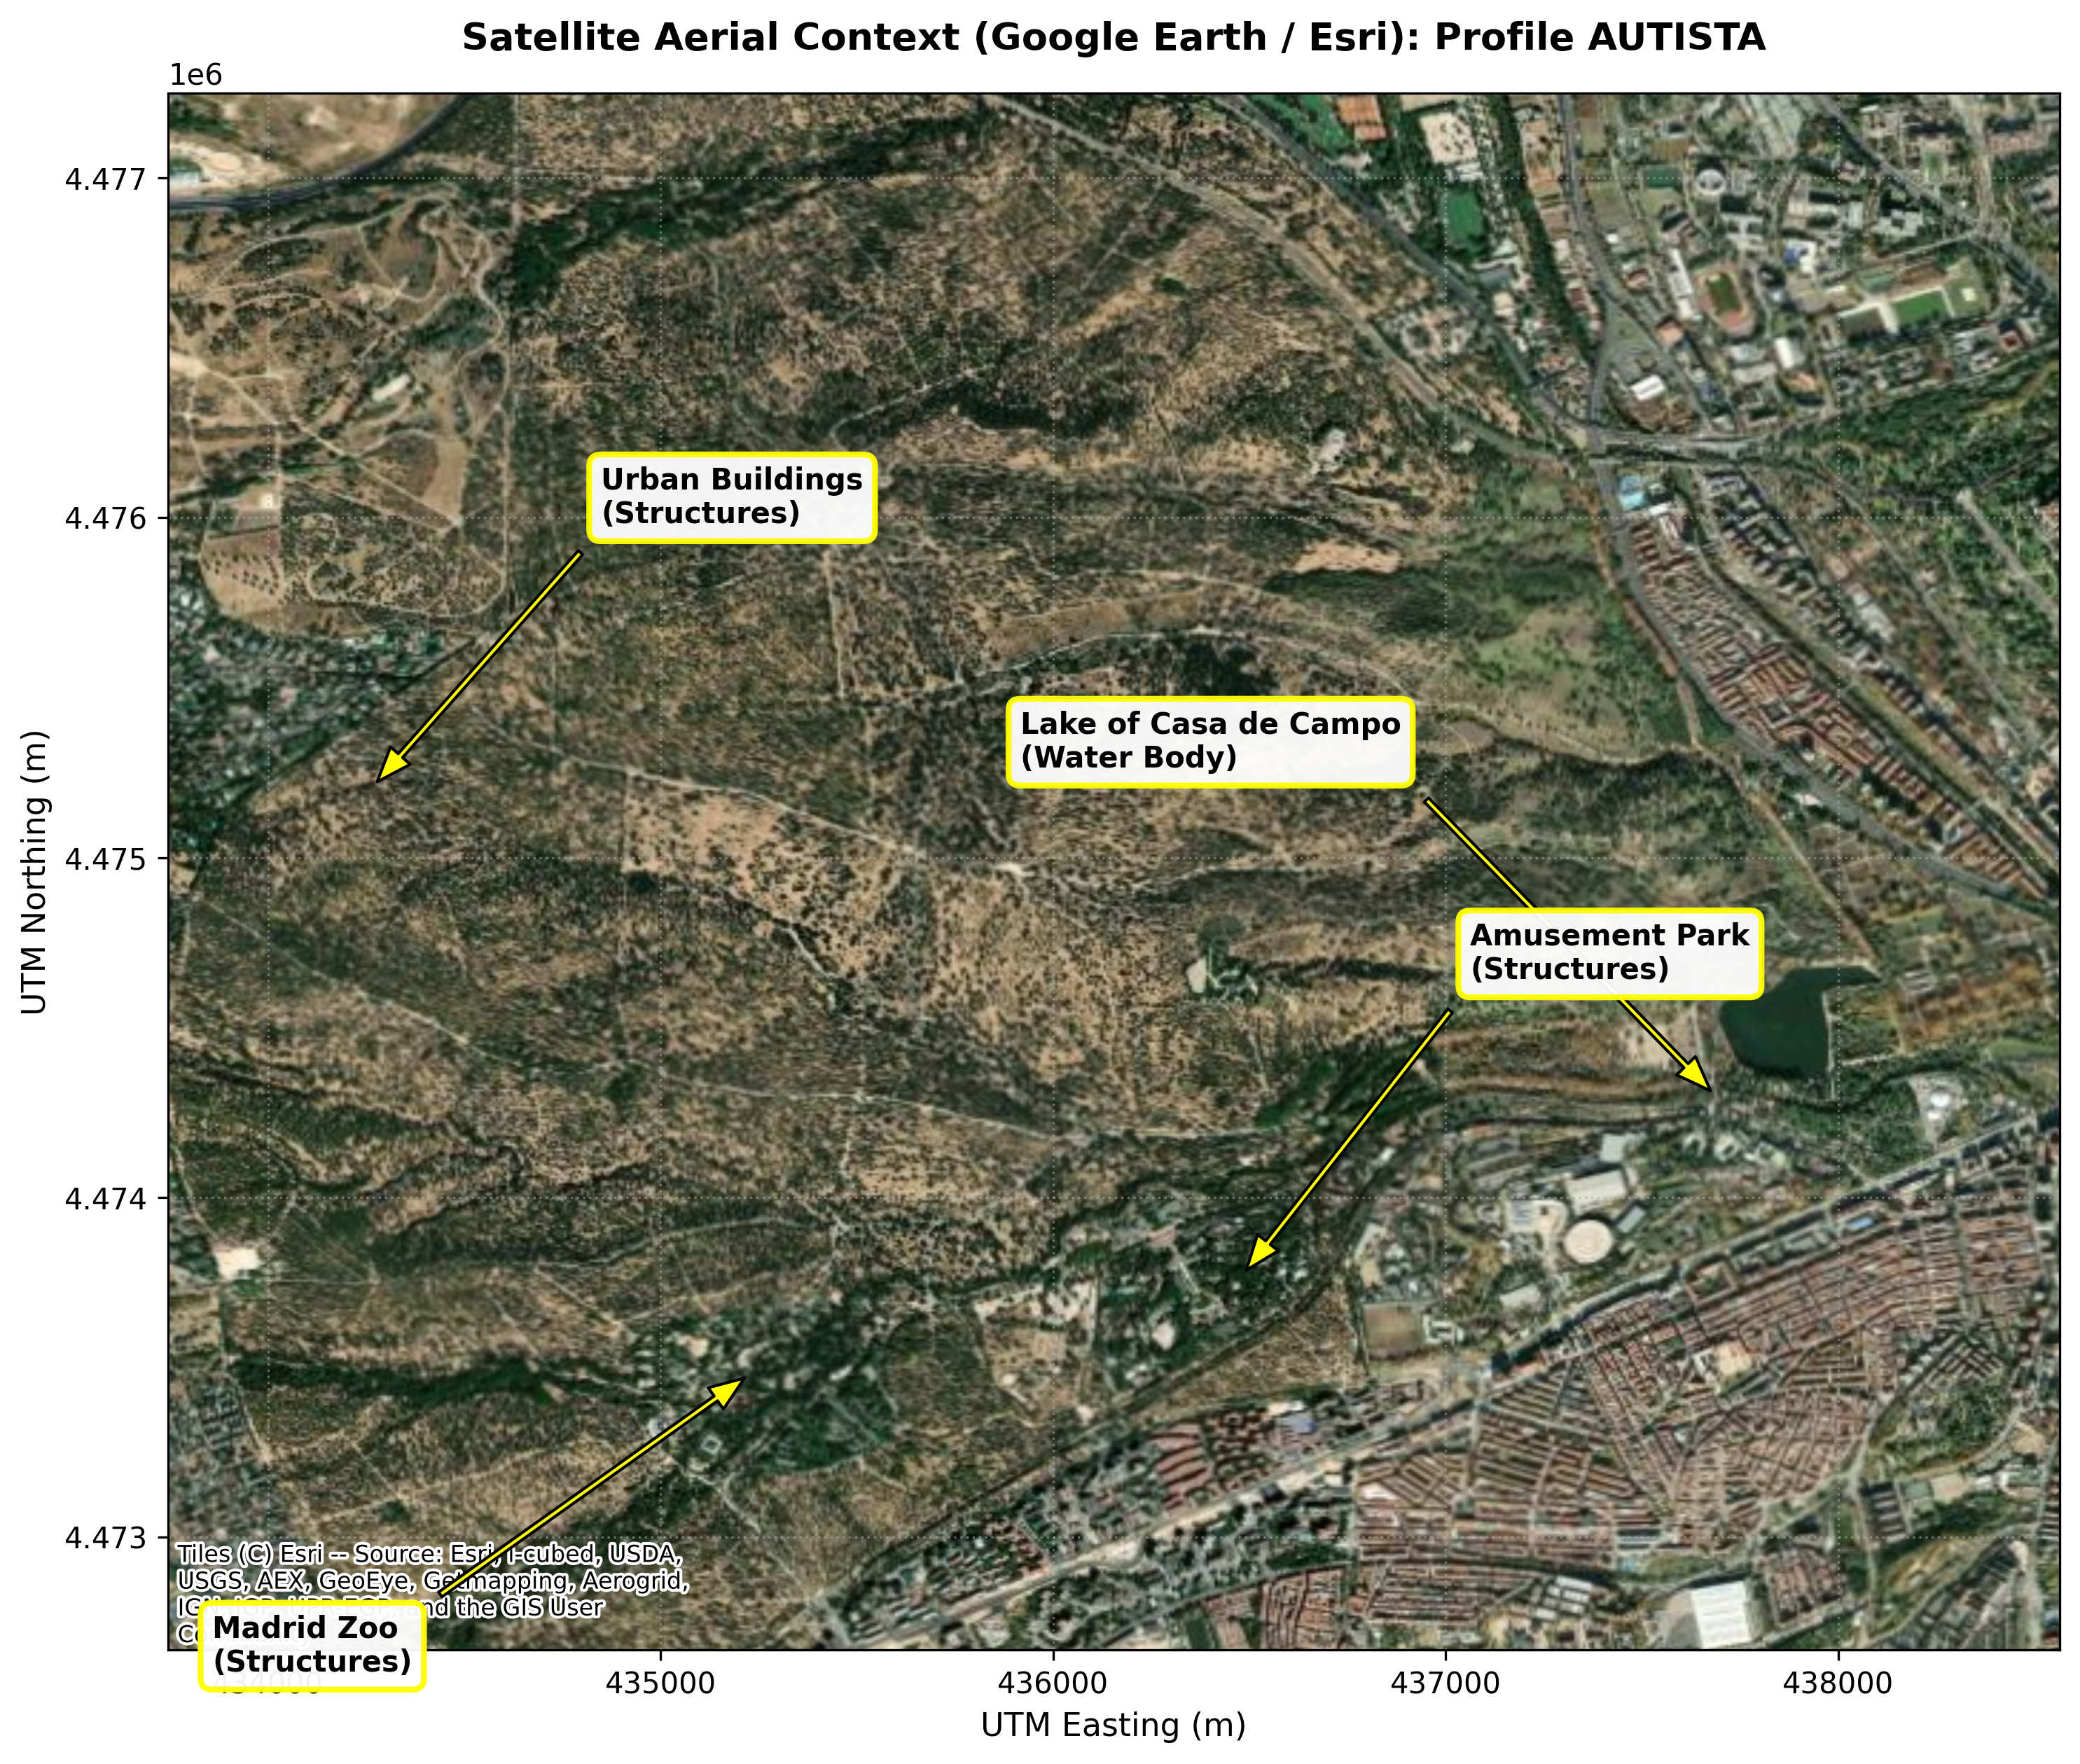
\includegraphics[width=0.95\textwidth]{imagenes/filtro_restricciones_satelite_autista.png}}
\end{figure}

\section{Observaciones y Modelo del Sensor (Sensor Ideal de Nivel 1)}

La capacidad del UAV para localizar a la víctima en el terreno se modela mediante el enfoque canónico de \textbf{Sensor Ideal de Huella Geométrica (Nivel 1)}, adaptado del modelo de observación desarrollado por Yago Brotón.

Bajo este modelo, la probabilidad de detección condicional $P_d(x,y \mid p_k)$ de una víctima ubicada en las coordenadas $(x,y)$ dada la posición del dron $p_k = (x_k, y_k)$ a una altitud de vuelo $h$ se define como una función determinista de cobertura binaria:
\begin{equation}
    P_d(x,y \mid p_k) = \begin{cases} 
        1.0 & \text{si } \sqrt{(x - x_k)^2 + (y - y_k)^2} \le R_d \\ 
        0.0 & \text{en otro caso} 
    \end{cases}
\end{equation}
donde $R_d$ representa el radio de cobertura efectiva de la cámara a bordo, el cual viene determinado por la altitud $h$ y el ángulo del campo de visión (\textit{Field of View - FoV}) $\theta_{\text{FoV}}$:
\begin{equation}
    R_d = h \cdot \tan\left(\frac{\theta_{\text{FoV}}}{2}\right)
\end{equation}

Para las condiciones nominales de vuelo en la Casa de Campo ($h = 50\text{ m}$ de altitud y $\theta_{\text{FoV}} = 90^\circ$), el radio de cobertura resultante en el suelo es exactamente $R_d = 50\text{ metros}$.

Dado el tamaño de celda de $10\text{ m} \times 10\text{ m}$, una huella circular de $R_d = 50\text{ m}$ cubre un radio discreto de 5 celdas a partir de la posición del dron. Si el centroide de una celda queda dentro de este radio de barrido, la celda se marca como observada y su probabilidad acumulada es absorbida por el dron.

\section{Filtro Recursivo Bayesiano (RBF) y Mapa de Creencias Residual}

Cuando un dron sobrevuela una región y no detecta a la víctima, esta observación negativa aporta información. El sistema debe reducir la probabilidad de presencia en las celdas observadas y, por conservación de la masa de probabilidad, aumentar proporcionalmente la probabilidad en el resto de las zonas no exploradas.

Este proceso de actualización dinámica de la matriz de creencias se implementa mediante el Filtro Recursivo Bayesiano. Denotemos como $b_t(i, j)$ la creencia (prior) de que la víctima está en la celda $(i, j)$ en el tiempo $t$. Si el dron inspecciona el área en el paso $t$ y la observación $y_t$ es negativa ($y_t = 0$, víctima no encontrada), la creencia actualizada para el paso $t+1$ se calcula aplicando el teorema de Bayes:
\begin{equation}
    b_{t+1}(i, j) = P\left(x = (i,j) \mid y_t = 0, b_t\right) = \frac{P\left(y_t = 0 \mid x = (i,j)\right) \cdot b_t(i, j)}{P\left(y_t = 0 \mid b_t\right)}
\end{equation}

Dado que bajo el sensor ideal $P\left(y_t = 1 \mid x = (i,j)\right) = P_d(i, j)$, la probabilidad de no detección condicional es $P\left(y_t = 0 \mid x = (i,j)\right) = 1 - P_d(i, j)$. La regla de actualización del RBF para cada celda $(i, j)$ es:
\begin{equation}
    b_{t+1}(i, j) = \frac{\left(1 - P_d(i, j)\right) \cdot b_t(i, j)}{1 - \sum_{u=1}^{N_y} \sum_{v=1}^{N_x} P_d(u, v) \cdot b_t(u, v)}
\end{equation}
Este filtro redistribuye dinámicamente la masa de probabilidad durante la simulación, guiando a los planificadores inteligentes hacia zonas no exploradas que aún conservan alta probabilidad de éxito.

\section{Simulación de Víctimas y Evaluación Estadística (Método de Montecarlo)}

Para validar la eficacia de los algoritmos de enrutamiento y estimar sus métricas de rendimiento reales, se requiere una validación matemática consistente. En el framework integrado, esto se implementa mediante simulaciones estadísticas de Montecarlo.

En un despliegue de rescate real, los drones buscan a \textbf{una única persona}. En la experimentación, simular $N = 50$ semillas independientes significa que el sistema ejecutará \textbf{50 misiones completas e independientes}:
\begin{itemize}
    \item \textbf{Punto Inicial Fijo de Despegue (LKP):} En todas las 50 ejecuciones, el dron despega de manera determinista desde el centro geométrico del parque o Punto de Planificación Inicial (LKP), reflejando el puesto de mando de emergencias.
    \item \textbf{Generación Estocástica de Víctimas:} En cada simulación $k \in \{1, \dots, 50\}$, el sistema genera de forma estocástica la ubicación de una sola víctima virtual $v_k$ en el mapa. Esta siembra se realiza mediante un muestreo ponderado sobre el mapa de calor $b(v^0)$ restringido a celdas transitables ($P > 0$).
    \item \textbf{Criterio de Descubrimiento:} Durante la simulación del universo $k$, se comprueba si la trayectoria del dron intercepta la huella del sensor de la víctima ($d \le 50\text{ m}$) en algún paso de tiempo. Si lo hace, la búsqueda se considera un \textbf{éxito} ($x_k = 1$). De lo contrario, es un fallo ($x_k = 0$).
\end{itemize}

\begin{figure}[H]
	\ffigbox[\FBwidth]
	{\caption{CROQUIS DE EVALUACIÓN MONTECARLO: DESPEGUE FIJO (LKP) Y MUESTREO DE VÍCTIMAS ESTOCÁSTICAS}}
	{\label{fig:croquis_montecarlo}
	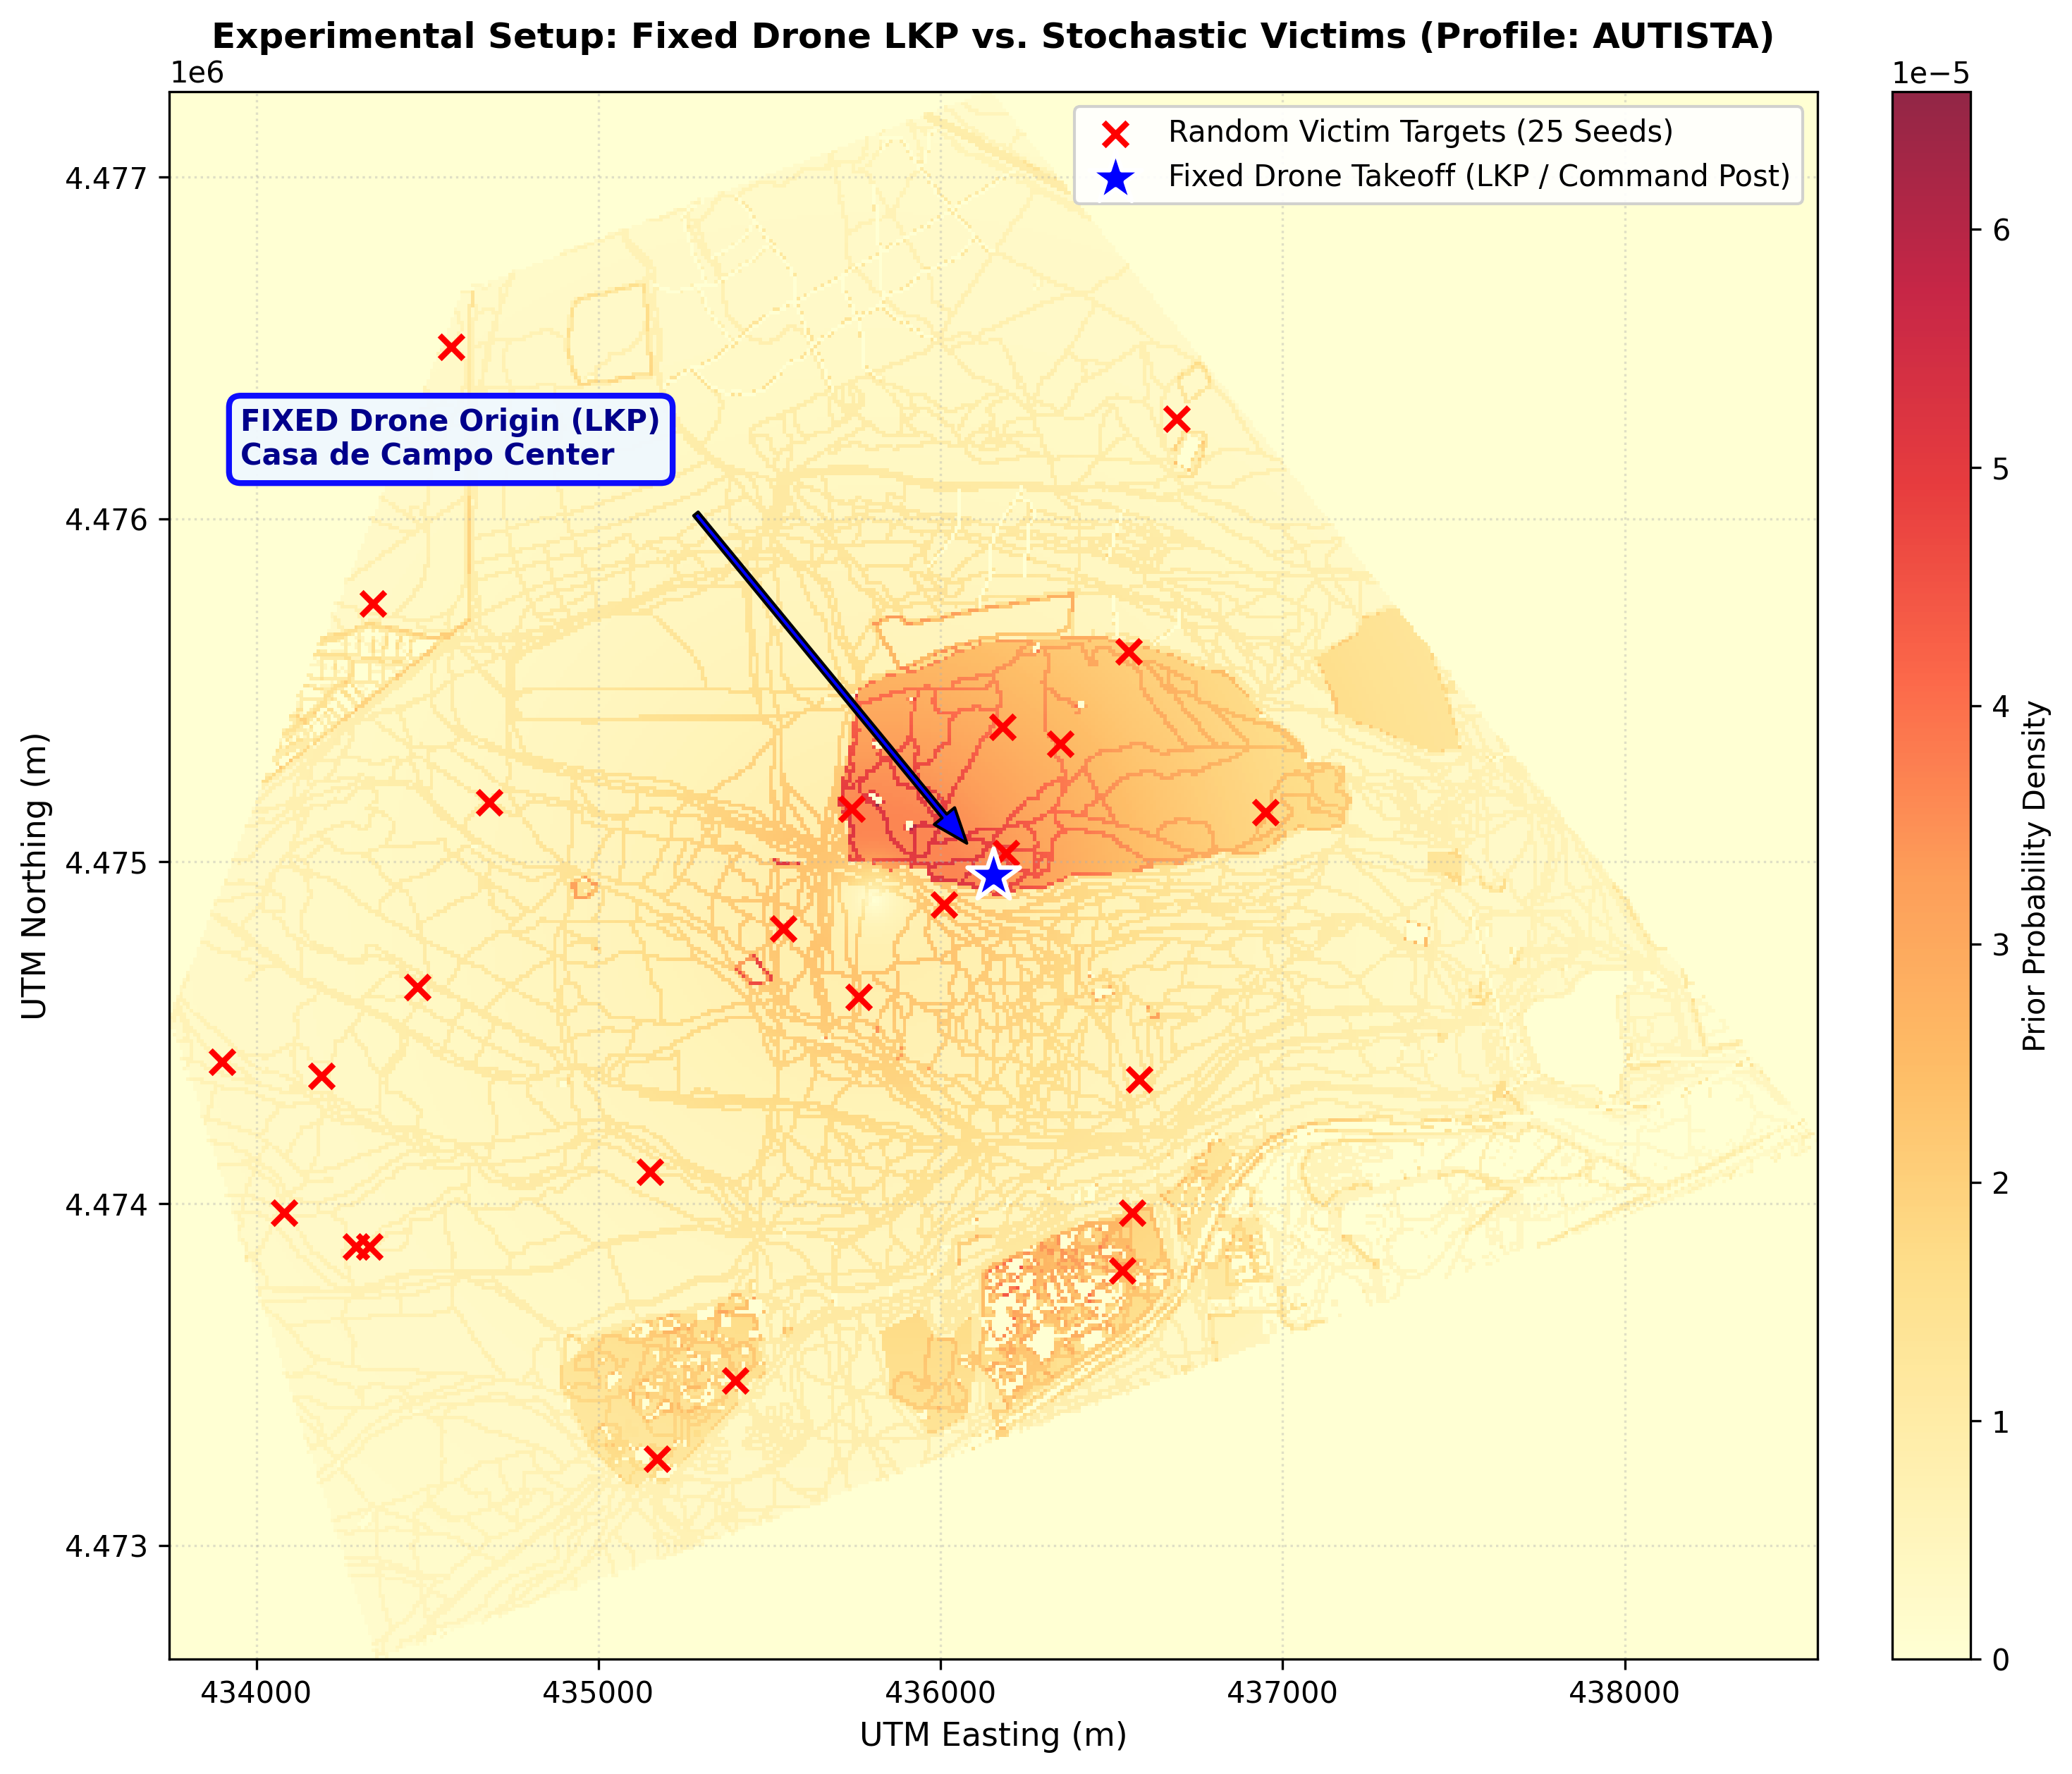
\includegraphics[width=0.90\textwidth]{imagenes/croquis_aleatoriedad_escenario.png}}
\end{figure}

El promedio de éxitos sobre las 50 simulaciones independientes define la métrica de éxito empírico:
\begin{equation}
    \text{Success Rate} = \frac{1}{N} \sum_{k=1}^{N} x_k
\end{equation}
Esta tasa acumulada proporciona robustez estadística, garantizando que el rendimiento reportado para un algoritmo no sea fruto de la suerte espacial de una única ejecución.

\chapter{Desarrollo del Framework e Integración Modular}
\label{ch:propuesta}

En este capítulo se presenta la arquitectura del framework desarrollado e integrado en este trabajo, denominado \texttt{sarenv-mts}. Se detalla la filosofía de diseño desacoplado del sistema, el flujo de datos entre sus cinco módulos constitutivos y la formulación matemática del middleware de transformación espacial.

\section{Arquitectura General de la Propuesta}

Para conectar de forma robusta la generación de mapas probabilísticos realistas basados en cartografía abierta con los motores de optimización de búsqueda en tiempo mínimo (MTS), se ha diseñado una arquitectura modular basada en cinco bloques funcionales independientes, ilustrada en la Figura~\ref{fig:diagrama_general}.

\begin{figure}[H]
	\ffigbox[\FBwidth]
	{\caption{DIAGRAMA DE ARQUITECTURA GENERAL DEL SISTEMA INTEGRADO SARENV-MTS}}
	{\label{fig:diagrama_general}
	\begin{tikzpicture}[node distance=1.8cm, auto,
	    block/.style={rectangle, draw=azulUC3M, fill=gray97, thick, text width=2.4cm, text centered, rounded corners, minimum height=1.3cm, font=\footnotesize\bfseries},
	    line/.style={draw=azulUC3M, thick, -latex}]
	    
	    \node [block] (m1) {Módulo 1\\Modelado Topológico\\(SAREnv \& LPB)};
	    \node [block, right of=m1, node distance=3.2cm] (m2) {Módulo 2\\Filtro de Restricciones\\(Sindex R-Tree)};
	    \node [block, right of=m2, node distance=3.2cm] (m3) {Módulo 3\\Middleware UTM\\(Proyección X,Y)};
	    \node [block, right of=m3, node distance=3.2cm] (m4) {Módulo 4\\Planificación MTS\\(ACO, ABC, BHA)};
	    \node [block, right of=m4, node distance=3.2cm] (m5) {Módulo 5\\Evaluador SAR\\(PathEvaluator)};
	    
	    \path [line] (m1) -- node[above, font=\tiny] {$POA_{\text{base}}$} (m2);
	    \path [line] (m2) -- node[above, font=\tiny] {$b(v^0)$} (m3);
	    \path [line] (m3) -- node[above, font=\tiny] {JSON / NPY} (m4);
	    \path [line] (m4) -- node[above, font=\tiny] {Trayectorias} (m5);
	\end{tikzpicture}}
\end{figure}

El diseño desacoplado garantiza que cada módulo opere como una pasarela independiente:
\begin{itemize}
    \item El modelado geográfico y probabilístico se calcula una sola vez de forma analítica en el Módulo 1.
    \item El enmascaramiento físico de seguridad y no transitabilidad se ejecuta en el Módulo 2.
    \item El Módulo 3 transforma las coordenadas globales en formato estándar JSON/Numpy compatible con el planificador.
    \item El Módulo 4 ejecuta la optimización bioinspirada de vuelo.
    \item El Módulo 5 realiza el análisis cuantitativo unificado de métricas SAR.
\end{itemize}

\section{Módulo 1: Generación de Cartografía y Probabilidad Espacial}

El primer módulo se encarga de descargar la geometría vectorial de OpenStreetMap y combinarla con el modelo probabilístico \textit{Lost Person Behavior} (LPB) de Robert Koester \cite{koester2008lost}.

\begin{figure}[H]
	\ffigbox[\FBwidth]
	{\caption{FLUJO DEL MÓDULO 1: GENERACIÓN DE PROBABILIDAD TOPOLÓGICA}}
	{\label{fig:diagrama_modulo1}
	\begin{tikzpicture}[node distance=1.5cm, auto,
	    block/.style={rectangle, draw=azulUC3M, fill=gray97, text width=3.8cm, text centered, rounded corners, minimum height=0.9cm, font=\footnotesize},
	    line/.style={draw=azulUC3M, thick, -latex}]
	    
	    \node [block] (osm) {Geometrías OSM (Casa de Campo)};
	    \node [block, below of=osm] (lpb) {Pesos Estadísticos por Perfil LPB};
	    \node [block, below of=lpb] (dist) {Dispersión Radial Log-Normal (LKP)};
	    \node [block, right of=lpb, node distance=5.5cm] (fusion) {\textbf{Suma Ponderada y Normalización}\\$\mathbf{POA}(i,j) = \frac{\sum_k \mathbf{M}_k \alpha_k}{\sum \mathbf{POA}}$};
	    \node [block, right of=fusion, node distance=4.5cm] (out1) {Matriz Base (.npy)};
	    
	    \path [line] (osm) -| (fusion);
	    \path [line] (lpb) -- (fusion);
	    \path [line] (dist) -| (fusion);
	    \path [line] (fusion) -- (out1);
	\end{tikzpicture}}
\end{figure}

Como se describió en el Capítulo 3, las capas semánticas (caminos, bosques, estructuras, agua, prados) se rasterizan en matrices binarias $\mathbf{M}_k$ y se combinan mediante una suma ponderada lineal, preservando los picos de verosimilitud de las intersecciones lineales.

\section{Módulo 2: Motor de Filtrado de Restricciones Físicas (\texttt{Sindex})}

El segundo módulo proyecta las geometrías de exclusión física (lagos profundos y edificaciones cerradas) sobre la rejilla espacial utilizando árboles de indexación jerárquica R-Tree (\texttt{sindex}), como se sintetiza en la Figura~\ref{fig:diagrama_modulo2}.

\begin{figure}[H]
	\ffigbox[\FBwidth]
	{\caption{FLUJO DEL MÓDULO 2: FILTRADO ESPACIAL DE RESTRICCIONES DURAS}}
	{\label{fig:diagrama_modulo2}
	\begin{tikzpicture}[node distance=1.5cm, auto,
	    block/.style={rectangle, draw=azulUC3M, fill=gray97, text width=3.8cm, text centered, rounded corners, minimum height=0.9cm, font=\footnotesize},
	    line/.style={draw=azulUC3M, thick, -latex}]
	    
	    \node [block] (in) {Matriz Base $\mathbf{POA}_{\text{base}}$};
	    \node [block, below of=in] (polys) {Polígonos No Transitables (Agua / Edificios)};
	    \node [block, right of=in, node distance=5.5cm] (mask) {\textbf{Máscara Espacial R-Tree}\\Anulación Estricta: $P(i,j) = 0.0$};
	    \node [block, below of=mask] (renorm) {Renormalización Global\\$\sum_{i,j} b(v^0)(i,j) = 1.0$};
	    \node [block, right of=mask, node distance=4.5cm] (out2) {Mapa de Creencias $b(v^0)$};
	    
	    \path [line] (in) -- (mask);
	    \path [line] (polys) -| (mask);
	    \path [line] (mask) -- (renorm);
	    \path [line] (renorm) -| (out2);
	\end{tikzpicture}}
\end{figure}

Este paso garantiza que los algoritmos de optimización reciban una distribución de probabilidad depurada $b(v^0)$, eliminando el desperdicio de batería sobre tejados o masas de agua y modelando una búsqueda aérea coordinada.

\section{Módulo 3: Middleware de Transformación de Coordenadas}

El tercer módulo actúa como pasarela matemática entre la cartografía georreferenciada global y la rejilla matricial discreta de simulación de MTS.

\begin{figure}[H]
	\ffigbox[\FBwidth]
	{\caption{FLUJO DEL MÓDULO 3: TRANSFORMACIÓN Y EXPORTACIÓN DEL MIDDLEWARE}}
	{\label{fig:diagrama_modulo3}
	\begin{tikzpicture}[node distance=1.5cm, auto,
	    block/.style={rectangle, draw=azulUC3M, fill=gray97, text width=4.0cm, text centered, rounded corners, minimum height=0.9cm, font=\footnotesize},
	    line/.style={draw=azulUC3M, thick, -latex}]
	    
	    \node [block] (utm) {Coordenadas UTM EPSG:32630\\$(x_{\min}, y_{\min}, x_{\max}, y_{\max})$};
	    \node [block, right of=utm, node distance=5.5cm] (trans) {\textbf{Transformación a Rejilla}\\$X = \lfloor \frac{\Delta x}{\delta} \rfloor, \quad Y = \lfloor \frac{\Delta y}{\delta} \rfloor$\\Resolución: $\delta = 10\text{ m}$};
	    \node [block, right of=trans, node distance=4.8cm] (json) {Escenario JSON / NPY\\Listo para MTS};
	    
	    \path [line] (utm) -- (trans);
	    \path [line] (trans) -- (json);
	\end{tikzpicture}}
\end{figure}

\subsection{Formulación Matemática de la Proyección de Coordenadas}

Sea el Punto de Planificación Inicial o punto de despegue $LKP = (\text{lon}_{\text{LKP}}, \text{lat}_{\text{LKP}})$. El middleware realiza los siguientes pasos:
\begin{enumerate}
    \item \textbf{Proyección Geográfica a UTM:} Se proyecta el par angular $(\text{lon}, \text{lat})$ a coordenadas métricas globales UTM Zona 30 Norte ($\text{EPSG:32630}$):
    \begin{equation}
        (x_{\text{UTM}}, y_{\text{UTM}}) = \mathcal{T}_{\text{WGS84}\to\text{UTM}}(\text{lon}_{\text{LKP}}, \text{lat}_{\text{LKP}})
    \end{equation}
    \item \textbf{Cálculo de Distancias Relativas al Origen del Escenario:} Sabiendo que el origen de la rejilla $(0,0)$ corresponde a la esquina inferior izquierda $(x_{\min}, y_{\min})$:
    \begin{equation}
        \Delta x = x_{\text{UTM}} - x_{\min}, \quad \Delta y = y_{\text{UTM}} - y_{\min}
    \end{equation}
    \item \textbf{Discretización a Índices Matriciales:} Dividiendo por la resolución espacial $\delta = 10\text{ m}$:
    \begin{equation}
        X_{\text{local}} = \left\lfloor \frac{\Delta x}{\delta} \right\rfloor, \quad Y_{\text{local}} = \left\lfloor \frac{\Delta y}{\delta} \right\rfloor
    \end{equation}
\end{enumerate}
El vector resultante $(X_{\text{local}}, Y_{\text{local}})$ define unívocamente la posición de despegue fija en la matriz discreta de MTS.

\subsection{Estructura de Intercambio del Escenario (\texttt{escenario.json})}

Para desacoplar el procesamiento cartográfico de la lógica de optimización, el middleware genera un archivo de configuración estandarizado en formato JSON vinculado a la matriz binaria \texttt{.npy}. Este fichero articula los parámetros cinemáticos, sensoriales y dimensionales de la misión:
\begin{itemize}
    \item \texttt{size}: Dimensiones matriciales de la rejilla $[N_x, N_y]$ ($458 \times 481$ celdas para la Casa de Campo).
    \item \texttt{init\_pos}: Vector de despegue $[[X_{\text{local}}, Y_{\text{local}}]]$ derivado del LKP.
    \item \texttt{posible\_moves}: Conectividad cinemática del UAV, fijada en 8 direcciones contiguas (vecindad de Moore: N, NE, E, SE, S, SW, W, NW).
    \item \texttt{num\_steps}: Presupuesto temporal de vuelo máximo ($T = 1000$ pasos por misión).
    \item \texttt{height} y \texttt{dmax}: Parámetros de altitud de crucero y huella sensorial efectiva ($R_d = 50\text{ m}$).
    \item \texttt{algoritmo\_busqueda}: Planificador seleccionado (\texttt{aco}, \texttt{abc}, \texttt{bha} o baselines de referencia).
\end{itemize}

\section{Módulo 4: Motor de Simulación y Algoritmos Bioinspirados (MTS)}

El Módulo 4 constituye el núcleo de enrutamiento deliberativo del sistema, integrando y extendiendo el framework \textit{MTS-UncertainEnvironment} \cite{Broton_Gutierrez_MTS-UncertainEnvironment}. A partir del mapa de creencias inicial $b(v^0)$ y las restricciones físicas calculadas en los módulos precedentes, el planificador genera trayectorias de vuelo optimizadas para interceptar a la víctima en tiempo mínimo.

\subsection{Formulación del Problema de Optimización de Trayectorias}

Sea $\mathcal{S} \subset \mathbb{Z}^2$ el espacio discreto de celdas de la rejilla y $\mathcal{M}$ el conjunto de movimientos admisibles de 8 conectividad. Una trayectoria para un UAV en un horizonte de tiempo $T$ se define como una secuencia ordenada de posiciones:
\begin{equation}
\pi = \left( p_0, p_1, p_2, \dots, p_T \right), \quad p_t \in \mathcal{S}, \quad p_{t+1} - p_t \in \mathcal{M}
\end{equation}
con $p_0 = (X_{\text{local}}, Y_{\text{local}})$. El objetivo del planificador es encontrar la trayectoria $\pi^*$ que maximice la ganancia acumulada de probabilidad de detección sobre el mapa dinámico de creencias $b(v^t)$ actualizado recursivamente mediante el RBF:
\begin{equation}
\pi^* = \arg\max_{\pi} \sum_{t=0}^{T} \sum_{(x,y) \in \text{FoV}(p_t)} b(v^t)(x, y)
\end{equation}
donde $\text{FoV}(p_t)$ denota el conjunto de celdas contenidas en la huella del sensor circular de radio $R_d = 50\text{ m}$ centrado en la posición $p_t$.

\subsection{Colonia de Hormigas (Ant Colony Optimization - ACO)}

La formulación de ACO en MTS implementa el esquema \textit{Max-Min Ant System} (MMAS) con feromona espacial 2D, adaptando los desarrollos de Carabaza et al. \cite{carabaza-ACOr, carabaza_ingles}:
\begin{enumerate}
    \item \textbf{Construcción Probabilística de Rutas:} Cada hormiga artificial construye una trayectoria desde $p_0$. La probabilidad de transición de la celda actual $i$ a la celda vecina $j \in \mathcal{N}(i)$ se rige por:
    \begin{equation}
    P_{ij} = \frac{[\tau_{ij}]^\alpha \cdot [\eta_{ij}]^\beta}{\sum_{l \in \mathcal{N}(i)} [\tau_{il}]^\alpha \cdot [\eta_{il}]^\beta}
    \end{equation}
    donde $\tau_{ij}$ representa la traza de feromona acumulada en el movimiento $i \to j$, y $\eta_{ij}$ es la deseabilidad heurística local, proporcional a la densidad de creencia $b(v^k)$ observable en el entorno de $j$. Los exponentes $\alpha$ y $\beta$ ponderan la influencia relativa del rastro histórico frente a la ganancia inmediata.
    \item \textbf{Evaporación y Depósito Acotado de Feromona:} Para evitar la convergencia prematura hacia óptimos locales, la feromona se evapora a una tasa $\rho \in (0,1)$, y solo la mejor hormiga global deposita nueva feromona $\Delta \tau$, acotando estrictamente los valores en el intervalo $[\tau_{\min}, \tau_{\max}]$:
    \begin{equation}
    \tau_{ij}(t+1) = \max \left( \tau_{\min}, \min \left( \tau_{\max}, (1-\rho)\tau_{ij}(t) + \Delta \tau_{ij}^{\text{best}} \right) \right)
    \end{equation}
\end{enumerate}

\subsection{Colonia de Abejas Artificiales (Artificial Bee Colony - ABC)}

El algoritmo ABC, adaptado a partir del paradigma original de Karaboga y Basturk \cite{karaboga2007}, modela la optimización de rutas mediante una población de fuentes de alimento (cada una representando una política o secuencia de decisiones de rumbo) gestionada por tres grupos de agentes:
\begin{enumerate}
    \item \textbf{Abejas Empleadas:} Cada abeja empleada está asociada a una trayectoria candidata $\mathbf{x}_i$. En cada iteración, explora las proximidades de su solución aplicando una perturbación estocástica:
    \begin{equation}
    v_{ij} = x_{ij} + \phi_{ij} (x_{ij} - x_{kj}), \quad \phi_{ij} \in [-1, 1]
    \end{equation}
    donde $k$ es otra solución seleccionada al azar. Si la nueva trayectoria produce una mayor absorción bayesiana, reemplaza a la anterior; en caso contrario, se incrementa un contador de estancamiento.
    \item \textbf{Abejas Observadoras:} Evalúan la calidad de todas las fuentes mediante un mecanismo de ruleta probabilística proporcional a su \textit{fitness} $J(\pi_i)$:
    \begin{equation}
    p_i = \frac{J(\pi_i)}{\sum_{m=1}^{SN} J(\pi_m)}
    \end{equation}
    Las observadoras concentran un mayor esfuerzo de refinamiento en las trayectorias que sobrevuelan zonas de alta densidad de personas extraviadas.
    \item \textbf{Abejas Exploradoras:} Si el contador de estancamiento de una fuente supera el umbral prefijado (\texttt{limit}), la solución se descarta por haberse agotado su margen de mejora local, y la abeja se transforma en exploradora, generando una nueva trayectoria en regiones inexploradas para mantener la diversidad del enjambre.
\end{enumerate}

\subsection{Algoritmo de Agujeros Negros (Black Hole Algorithm - BHA)}

Inspirado en la mecánica gravitatoria cósmica formulada por Hatamlou \cite{hatamlou2012}, BHA opera sobre una población de $N_{\text{stars}}$ trayectorias candidatas denominadas estrellas:
\begin{enumerate}
    \item \textbf{Identificación del Agujero Negro:} La trayectoria con mayor valor de absorción de probabilidad acumulada es designada como el Agujero Negro central ($\mathbf{X}_{BH}$).
    \item \textbf{Atracción Gravitacional de Soluciones:} En cada paso del algoritmo, todas las estrellas son atraídas hacia la trayectoria líder modificando sus vectores de decisión:
    \begin{equation}
    \mathbf{X}_i(t+1) = \mathbf{X}_i(t) + \mathbf{r} \cdot \left( \mathbf{X}_{BH} - \mathbf{X}_i(t) \right)
    \end{equation}
    donde $\mathbf{r}$ es un vector aleatorio con distribución uniforme en $[0, 1]$. Si una estrella supera en \textit{fitness} al agujero negro actual, asume inmediatamente el rol de nuevo agujero negro.
    \item \textbf{Horizonte de Sucesos y Regeneración Estocástica:} Para evitar el colapso prematuro de la población en un único punto, se define el radio del horizonte de sucesos (análogo al radio de Schwarzschild):
    \begin{equation}
    R_{EH} = \frac{J(\mathbf{X}_{BH})}{\sum_{i=1}^{N_{\text{stars}}} J(\mathbf{X}_i)}
    \end{equation}
    Cualquier estrella cuya distancia euclídea al agujero negro sea inferior a $R_{EH}$ se considera absorbida, destruida y regenerada aleatoriamente en el espacio de búsqueda.
\end{enumerate}

\subsection{Planificadores Clásicos de Referencia (Baselines)}

Para contrastar el beneficio de los métodos bioinspirados frente a las estrategias estándar de rescate, el Módulo 4 incorpora tres algoritmos clásicos:
\begin{itemize}
    \item \textbf{Búsqueda Voraz (\textit{Greedy}):} En cada celda $p_t$, el UAV evalúa sus 8 vecinos admisibles y avanza hacia aquel con la mayor densidad de creencia $b(v^t)$, sin planificación a largo plazo.
    \item \textbf{Patrón Boustrophedon (\textit{Lawnmower}):} Cobertura geométrica sistemática en pasadas paralelas de ida y vuelta, cubriendo exhaustivamente el terreno sin guiado probabilístico.
    \item \textbf{Espiral Expansiva (\textit{Expanding Spiral}):} Trayectoria geométrica de radios crecientes centrada en el LKP, representativa de las búsquedas visuales manuales en rescate tradicional.
\end{itemize}

\section{Módulo 5: Evaluador Centralizado de Métricas SAR (\texttt{PathEvaluatorTFM})}

El Módulo 5 centraliza la evaluación cuantitativa independiente de todas las trayectorias generadas, aplicando el estándar del módulo \texttt{PathEvaluatorTFM}:

\begin{figure}[H]
	\ffigbox[\FBwidth]
	{\caption{FLUJO DEL MÓDULO 5: EVALUACIÓN UNIFICADA DE RENDIMIENTO SAR}}
	{\label{fig:diagrama_modulo5}
	\begin{tikzpicture}[node distance=1.5cm, auto,
	    block/.style={rectangle, draw=azulUC3M, fill=gray97, text width=3.8cm, text centered, rounded corners, minimum height=0.9cm, font=\footnotesize},
	    line/.style={draw=azulUC3M, thick, -latex}]
	    
	    \node [block] (traj) {Trayectoria $(X,Y)$ y Telemetría CSV};
	    \node [block, below of=traj] (map) {Mapa de Creencias Base $b(v^0)$};
	    \node [block, right of=traj, node distance=5.5cm] (eval) {\textbf{PathEvaluatorTFM}\\Cálculo Vectorial Shapely / RBF};
	    \node [block, right of=eval, node distance=4.5cm] (metrics) {5 Métricas SAR Oficiales (CSV / Boxplots)};
	    
	    \path [line] (traj) -- (eval);
	    \path [line] (map) -| (eval);
	    \path [line] (eval) -- (metrics);
	\end{tikzpicture}}
\end{figure}

Las cinco métricas evaluadas son:
\begin{enumerate}
    \item \textbf{Tasa de Éxito (\textit{Success Rate}, \%):} Porcentaje de misiones en las que el dron intercepta la víctima virtual a una distancia $d \le 50\text{ m}$.
    \item \textbf{Pasos hasta el Hallazgo (\textit{Steps to Goal}):} Número de instantes temporales transcurridos hasta la detección.
    \item \textbf{Probabilidad Acumulada Absorbida (\textit{Reduced Belief}, \%):} Fracción de la masa de probabilidad total del mapa eliminada tras el paso del sensor.
    \item \textbf{Área Geográfica Barrida (\textit{Covered Area}, $\text{km}^2$):} Superficie neta cubierta por la huella del sensor sin duplicar solapamientos.
    \item \textbf{Distancia de Vuelo (\textit{Total Flight Length}, km):} Longitud métrica total de la trayectoria recorrida.
\end{enumerate}

\section{Herramientas de Control y Validación Interactiva (Jupyter Notebooks)}

Para facilitar la experimentación, inspección visual y demostración en tiempo real de los algoritmos, se ha desarrollado un conjunto de cuadernos interactivos en Jupyter (\texttt{Notebook\_Demo\_Rapida\_Interactiva.ipynb}), cuya interfaz dual se ilustra en la Figura~\ref{fig:demo_interactiva}.

\begin{figure}[H]
	\ffigbox[\FBwidth]
	{\caption{PANEL DUAL DE SIMULACIÓN Y MÉTRICAS EN TIEMPO REAL (DEMO INTERACTIVA)}}
	{\label{fig:demo_interactiva}
	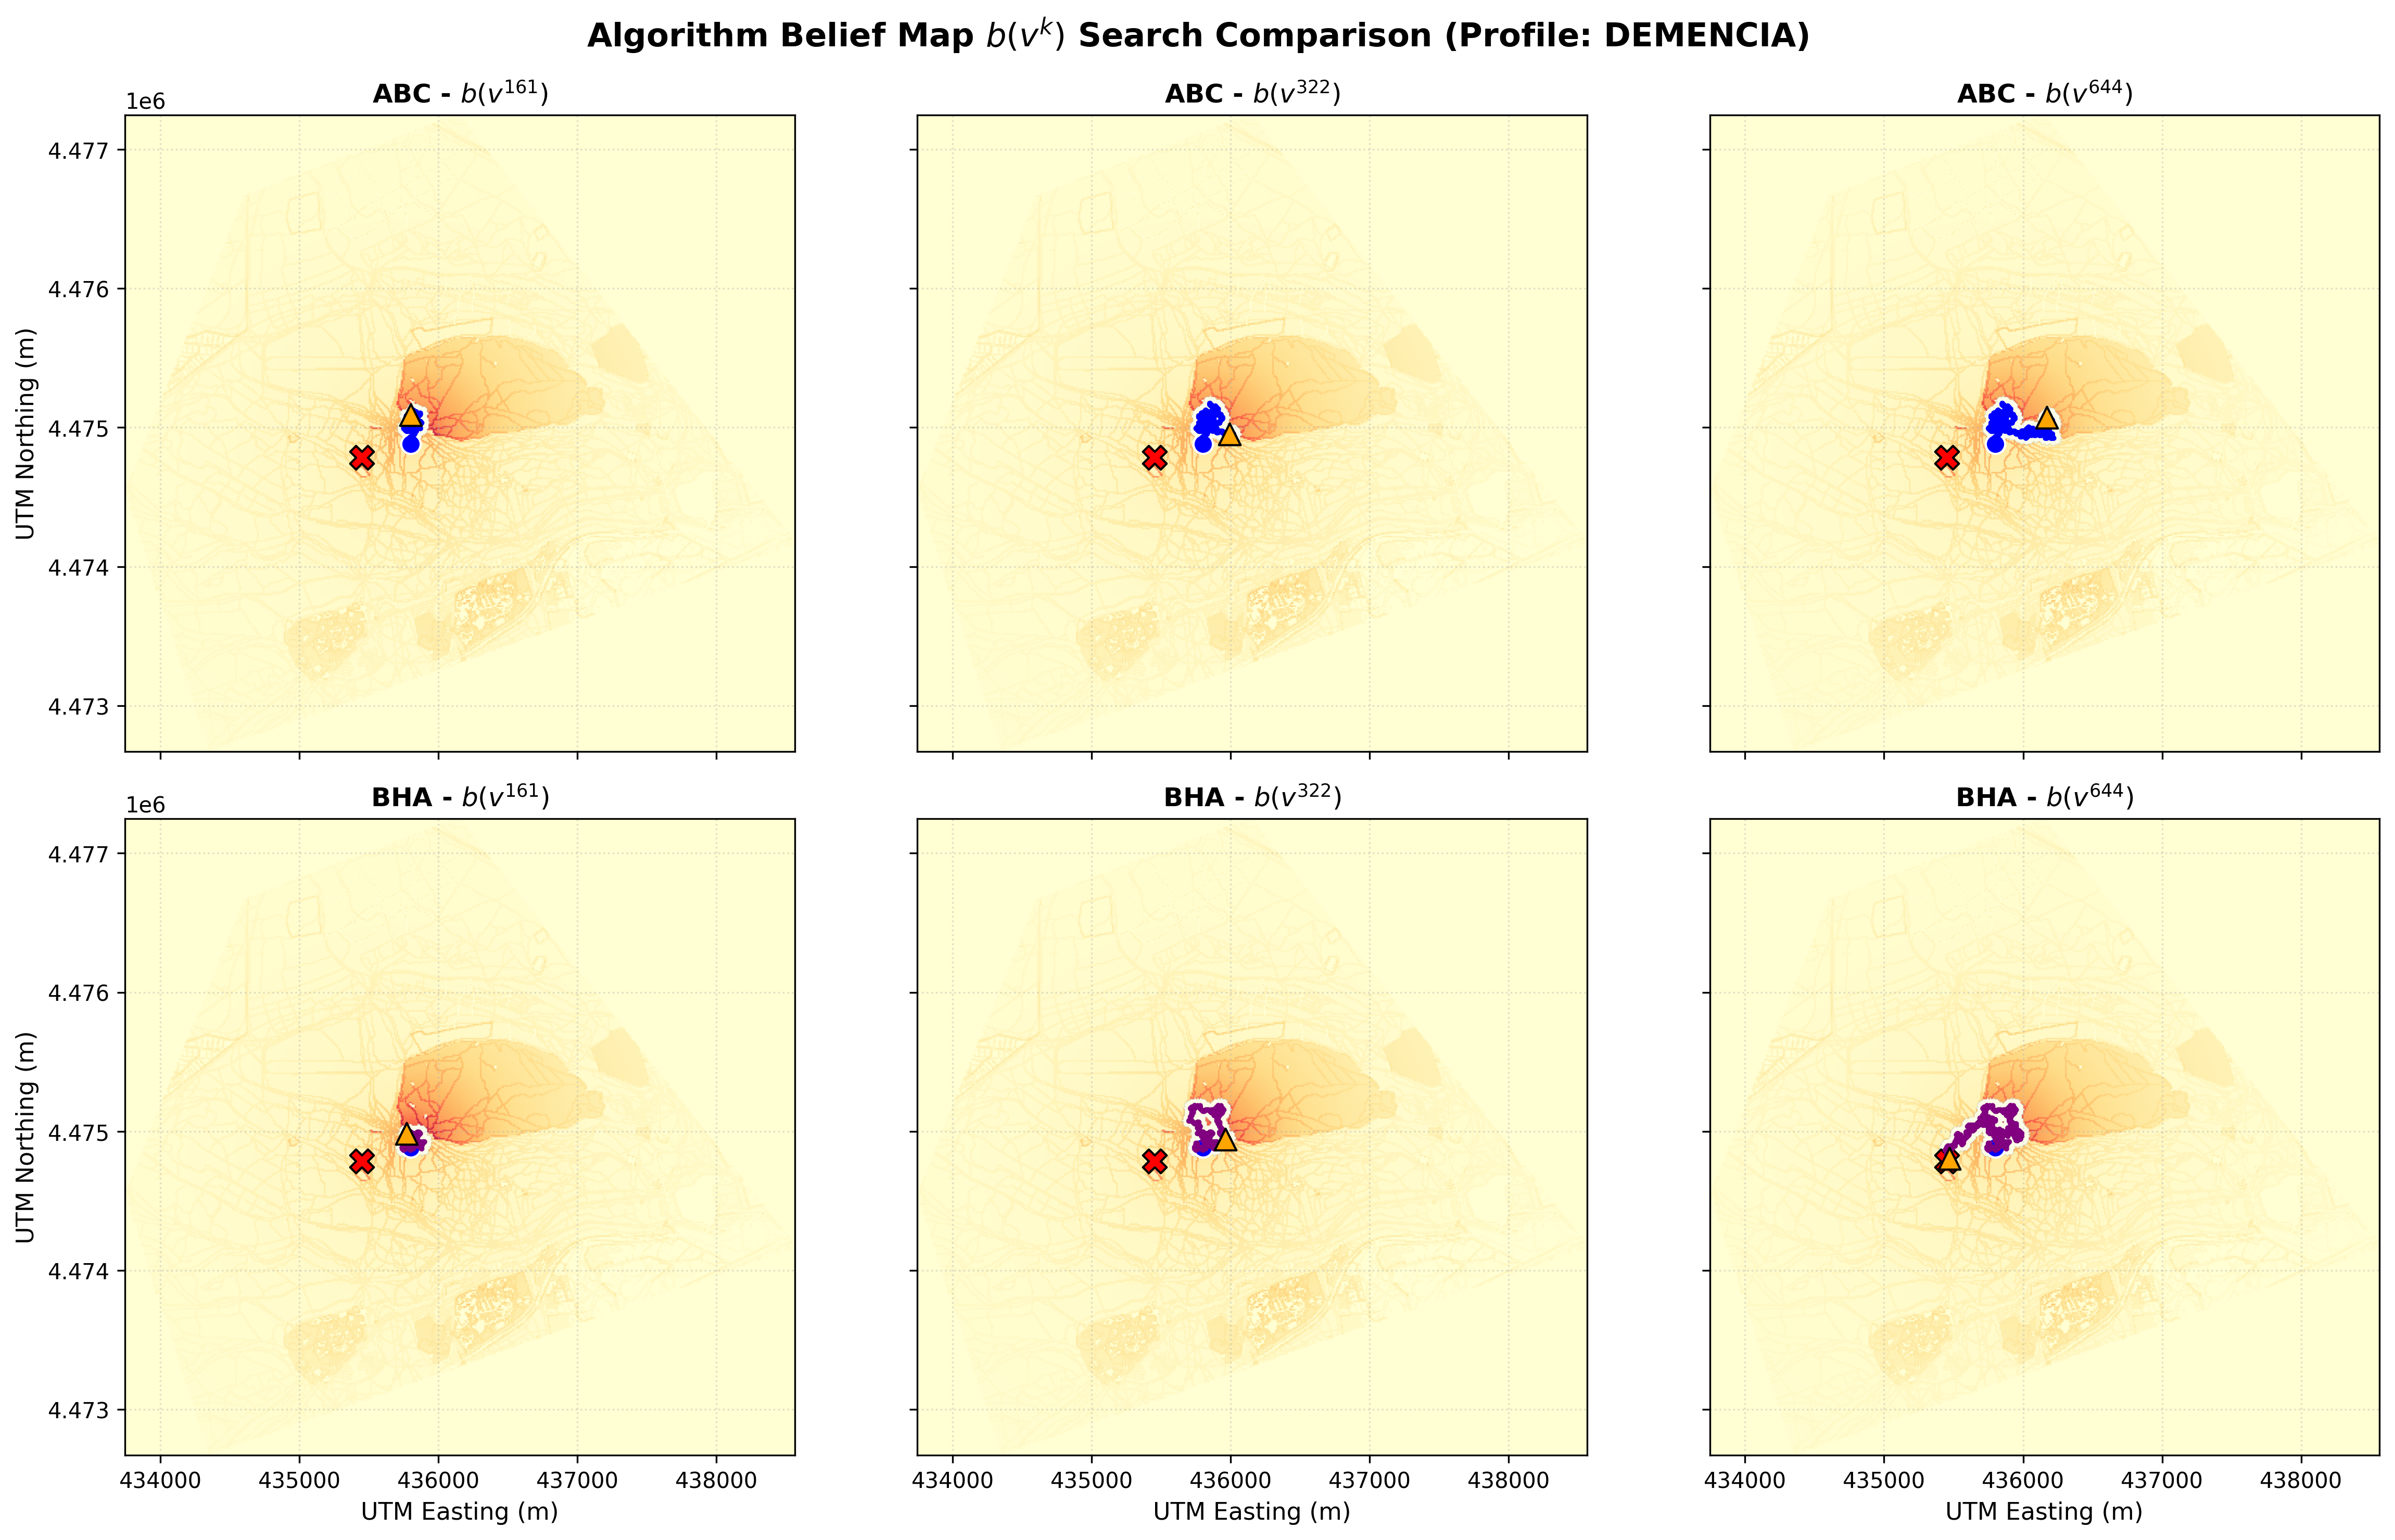
\includegraphics[width=0.95\textwidth]{imagenes/comparativa_evolucion_demencia_abc_vs_bha.png}}
\end{figure}

Esta herramienta permite al operador seleccionar de forma interactiva el perfil de la víctima, visualizar el mapa de calor con restricciones, seleccionar el algoritmo deseado y observar instantáneamente tanto la trayectoria volada como el mapa de creencias residual $b(v^{\text{Final}})$ con su correspondiente cuadro de métricas SAR.

\chapter{Proceso de Experimentación}

En este capítulo se expone el diseño experimental planteado para comparar el rendimiento de los planificadores metaheurísticos propuestos frente a las líneas de base tradicionales. Para dotar a las pruebas de realismo y validez académica, la experimentación se fundamenta en las estadísticas reales de comportamiento de personas perdidas (\textit{Lost Person Behavior} o LPB) y en las métricas de evaluación formales del simulador SAREnv.

\section{Diseño del Banco de Pruebas: Escenarios Canónicos y LPB}

Para la evaluación rigurosa de los algoritmos de planificación de trayectorias con UAVs, resulta indispensable contar con un escenario base o \textit{Ground Truth} que no dependa de distribuciones aleatorias ad-hoc, sino de modelados basados en el comportamiento real humano. El framework SAREnv fundamenta su modelo de probabilidad en los estudios estadísticos de comportamiento de personas perdidas (\textit{Lost Person Behavior} o LPB) desarrollados por Koester. En lugar de realizar una búsqueda uniforme, el sistema emplea la cartografía vectorial de OpenStreetMap para generar una Matriz de Probabilidades (MAP o \textit{Heatmap}) que prioriza los sectores de búsqueda.

\subsection{Probabilidad Espacial: Cuartiles de Distancia al LKP}

El primer componente estadístico del modelo LPB define el límite geográfico de la búsqueda a partir de la distancia recorrida desde el punto de planificación o LKP (\textit{Last Known Point}). Para el caso de estudio de la Casa de Campo, clasificado como un entorno llano y de clima templado (\textit{flat temperate}), el framework aplica internamente las siguientes distancias estadísticas de dispersión:
\begin{itemize}
    \item \textbf{Radio Small (0.6 km):} Abarca el 25\% de los casos históricos de dispersión.
    \item \textbf{Radio Medium (1.8 km):} Abarca el 50\% de los casos históricos de dispersión (mediana).
    \item \textbf{Radio Large (3.2 km):} Abarca el 75\% de los casos históricos de dispersión.
    \item \textbf{Radio XLarge (9.9 km):} Abarca el 95\% de los casos de dispersión.
\end{itemize}

\subsection{Probabilidad Topológica y Fusión de Capas}

Basándose en la tabla de probabilidades climáticas del LPB, la ponderación porcentual asignada a las capas cartográficas varía significativamente dependiendo de si el entorno es templado o seco. En la Tabla \ref{tab:probabilidades_clima} se detallan los pesos asignados a cada una de las características geográficas vectorizadas en función del tipo de clima.

\begin{table}[H]
	\ttabbox[\FBwidth]
	{\caption{PONDERACIÓN PROBABILÍSTICA DE LAS CAPAS CARTOGRÁFICAS SEGÚN EL CLIMA EN EL MODELO LPB}}
	{\label{tab:probabilidades_clima}
	\begin{tabular}{|l|c|c|}
		\hline
		\textbf{Característica Geográfica (Capa)} & \textbf{Ponderación Clima Templado} & \textbf{Ponderación Clima Seco} \\
		\hline
		Elementos lineales (vallas, vías) & 25\% & 31\% \\
		\hline
		Campo abierto (\textit{Field}) & 14\% & 1\% \\
		\hline
		Caminos y carreteras (\textit{Road}) & 13\% & 17\% \\
		\hline
		Estructuras (\textit{Building}) & 13\% & 10\% \\
		\hline
		Drenajes y arroyos (\textit{Drainage}) & 12\% & 18\% \\
		\hline
		Masas de agua (\textit{Water}) & 8\% & 9\% \\
		\hline
		Bosques (\textit{Woodland}) & 7\% & 6\% \\
		\hline
		Rocas & 4\% & 2\% \\
		\hline
		Matorral ralo (\textit{Scrub}) & 3\% & 3\% \\
		\hline
		Matorral denso (\textit{Brush}) & 2\% & 2\% \\
		\hline
		\multicolumn{3}{l}{Fuente: Datos estadísticos de Lost Person Behavior (Koester).}
	\end{tabular}}
\end{table}

Para generar el mapa de calor final, las geometrías son rasterizadas en matrices binarias y multiplicadas por los pesos descritos en la Tabla \ref{tab:probabilidades_clima}. En caso de solapamiento de capas, el framework no realiza una suma de probabilidades, sino que emplea una fusión por máximos mediante el operador de máximo elemento a elemento (\enquote{\texttt{np.maximum}}), garantizando que cada sector herede estrictamente la probabilidad de la característica geográfica más relevante.

\subsection{Definición de Escenarios Canónicos y Perfiles de Víctimas}

La evaluación de los algoritmos de búsqueda bioinspirados (Colonia de Hormigas, Enjambre de Abejas y Agujeros Negros) se realiza sobre escenarios que replican situaciones operativas reales en el entorno de la Casa de Campo de Madrid. A partir de los datos recopilados en la literatura y de la parametrización probabilística explicada, se definen tres escenarios canónicos que modelan perfiles específicos de víctimas:

\begin{enumerate}
    \item \textbf{Escenario A: Perfil de Demencia (Alzheimer):}
    \begin{itemize}
        \item \textbf{Justificación LPB:} Las personas con demencia senil o enfermedad de Alzheimer suelen presentar una desorientación cognitiva severa acompañada de limitaciones físicas de movilidad. Estadísticamente, la distancia de dispersión desde el punto de planificación o LKP (\textit{Last Known Point}) es reducida, concentrándose la gran mayoría de los casos en un radio muy cercano. En SAREnv, esto se modela utilizando un radio de búsqueda \enquote{small} ($0.6$~km), equivalente al percentil 25 de dispersión.
        \item \textbf{Comportamiento y Capas:} Estas víctimas tienden a seguir la ley del mínimo esfuerzo físico, desviándose con facilidad de los senderos pavimentados y quedando frecuentemente atrapadas en zonas de vegetación densa (bosques, matorrales) o cerca de estructuras aisladas. En la fusión bayesiana, se asignan pesos elevados a las capas de coberturas de bosques (\textit{woodland}) y matorrales (\textit{brush}), y nulos o muy bajos a la red vial activa, forzando un mapa de probabilidad concentrado en el arbolado y estructuras cercanas al LKP.
    \end{itemize}

    \item \textbf{Escenario B: Perfil de Senderista (Hiker):}
    \begin{itemize}
        \item \textbf{Justificación LPB:} Los senderistas o excursionistas perdidos disponen de plena capacidad física e intención de desplazarse a través del terreno. Por ende, la distancia de dispersión con respecto al LKP es sustancialmente mayor. Se utiliza el radio de búsqueda \enquote{large} ($3.2$~km), representativo del percentil 75 en las estadísticas de LPB.
        \item \textbf{Comportamiento y Capas:} El movimiento del senderista está fuertemente condicionado por la infraestructura lineal disponible. Suelen seguir caminos, senderos y pistas forestales en su intento de orientarse o regresar. Para este perfil, la capa lineal de la red de caminos (\textit{road} y \textit{linear}) recibe la ponderación preponderante en la fusión bayesiana de SAREnv. Esto produce un mapa de probabilidad de distribución alargado a lo largo de las vías de comunicación de la Casa de Campo.
    \end{itemize}

    \item \textbf{Escenario C: Escenario Dinámico (Víctima Móvil):}
    \begin{itemize}
        \item \textbf{Justificación LPB y Dinámica:} En muchas situaciones reales de emergencia, la persona extraviada no permanece estática, sino que continúa caminando de forma errática o siguiendo una dirección preferente. Esto altera dinámicamente la distribución espacial de la probabilidad de encontrar a la víctima a lo largo de la misión.
        \item \textbf{Modelado en MTS:} Aprovechando las capacidades de simulación del framework MTS (\textit{Multi-Agent Target Search}), se introduce una matriz de probabilidad de transición espacial $P_{\text{transicion}}$. La víctima inicia su posición en una celda central según el mapa bayesiano de SAREnv y, en cada paso temporal del dron, su posición evoluciona estocásticamente siguiendo una caminata aleatoria restringida por las coberturas transitables del terreno.
    \end{itemize}
\end{enumerate}


\section{Variables y Parámetros Controlados}

Para asegurar una comparativa justa (\textit{benchmark}) entre las estrategias heurísticas y de base, se fijan de forma rigurosa los siguientes parámetros experimentales en el middleware y en el entorno de simulación:

\begin{itemize}
    \item \textbf{Número de agentes búsqueda:} Se configura un único vehículo aéreo no tripulado (dron) de búsqueda para simplificar el análisis y evitar problemas ajenos al enrutamiento como la colisión de agentes en el simulador MTS.
    \item \textbf{Presupuesto de movimiento (\textit{budget}):} Limitado a un número fijo de pasos o distancia de vuelo equivalente a la capacidad nominal de la batería de un dron comercial estándar (estimada en $30$ minutos de vuelo).
    \item \textbf{Altitud de vuelo ($H$):} Fijada de forma constante en $50$ metros sobre el nivel del suelo, equilibrando el campo de visión de la cámara con la resolución necesaria para la detección de personas.
    \item \textbf{Parámetros del sensor a bordo:} Se asume una cámara con un campo de visión angular (FOV) de $90^{\circ}$, lo que determina un radio de detección física de la víctima $R_{\text{det}}$ a partir de la proyección cónica del sensor:
    \begin{equation}
        R_{\text{det}} = H \cdot \tan\left(\frac{\theta_{\text{FOV}}}{2}\right) = 50 \cdot \tan(45^{\circ}) = 50 \text{ metros}
    \end{equation}
    \item \textbf{Resolución del mapa:} Un tamaño de celda en el grid de probabilidad de $10 \times 10$ metros para garantizar tanto el detalle geográfico de la Casa de Campo como la eficiencia en el cálculo computacional.
\end{itemize}

\section{Metodología de Validación y Métricas de Rendimiento}

Dada la naturaleza estocástica de los algoritmos metaheurísticos de planificación (como la selección probabilística en ACO y las perturbaciones aleatorias en ABC y BHA), resulta indispensable validar los resultados estadísticamente. Para cuantificar la eficacia empírica de las trayectorias planificadas, el framework emplea un método de evaluación por simulación de Montecarlo distribuyendo virtualmente una muestra de $100$ víctimas independientes por el entorno. Estas posiciones de víctimas objetivo se \enquote{siembran} en el área obedeciendo estrictamente a la densidad topológica de la Matriz de Probabilidades (MAP). Por consiguiente, los agentes de búsqueda son evaluados en función de su eficiencia para maximizar el consumo de probabilidad acumulada y localizar estadísticamente el mayor número de estas víctimas sembradas.

Adicionalmente, para capturar la variabilidad de las heurísticas de enrutamiento, cada simulación de búsqueda sobre los escenarios canónicos se repite a lo largo de $50$ ejecuciones independientes (Montecarlo global). Esto permite obtener valores medios y desviaciones típicas robustas de cada una de las métricas de rendimiento y realizar comparaciones estadísticas significativas.

Para la evaluación formal de las trayectorias de búsqueda generadas por los algoritmos, se adoptan las cinco métricas académicas implementadas en el módulo \texttt{PathEvaluator} de SAREnv, garantizando una comparación matemáticamente consistente con la literatura científica:

\begin{enumerate}
    \item \textbf{Probabilidad de Detección Acumulada (\textit{Likelihood Score} - $S_{\text{like}}$):}
    Representa la suma de los valores de probabilidad de todas las celdas del mapa de calor que han sido observadas al menos una vez por el sensor del dron a lo largo del recorrido. Si definimos el conjunto de todas las celdas únicas cubiertas por la proyección del sensor a lo largo de la trayectoria como $\mathcal{C}_{\text{obs}}$, la métrica se define como:
    \begin{equation}
        S_{\text{like}} = \sum_{(r,c) \in \mathcal{C}_{\text{obs}}} \mathcal{M}_{r,c}
    \end{equation}
    donde $\mathcal{M}_{r,c}$ es el valor de la probabilidad en la celda situada en la fila $r$ y columna $c$ de la matriz del mapa de calor, normalizada tal que $\sum_{r,c} \mathcal{M}_{r,c} = 1.0$.

    \item \textbf{Puntuación Descontada por Tiempo (\textit{Time-Discounted Score} - $S_{\text{td}}$):}
    En misiones SAR, localizar a la víctima de forma temprana es crítico para su supervivencia. Esta métrica introduce un factor de descuento geométrico $\gamma \in (0, 1]$ que penaliza la demora en visitar las zonas de alta probabilidad. Para cada instante temporal de la trayectoria a una distancia acumulada $d(t)$, se evalúan las celdas visibles $\mathcal{V}(x(t))$:
    \begin{equation}
        S_{\text{td}} = \sum_{t} \left( \sum_{(r,c) \in \mathcal{V}(x(t))} \mathcal{M}_{r,c} \right) \cdot \gamma^{d(t)}
    \end{equation}
    donde $d(t)$ actúa como proxy del tiempo transcurrido y $\gamma$ se fija por defecto en $0.999$ por metro de avance.

    \item \textbf{Porcentaje de Víctimas Localizadas ($P_{\text{found}}$):}
    Mide el porcentaje de acierto de localización sobre un conjunto de víctimas estocásticas situadas en el entorno según la distribución de probabilidad subyacente. Si la trayectoria del dron se denota como el conjunto de puntos $P$ y definimos el área de cobertura efectiva mediante la unión de buffers de detección de radio $R_{\text{det}}$:
    \begin{equation}
        \mathcal{A}_{\text{eff}} = \bigcup_{p \in P} \mathcal{B}(p, R_{\text{det}})
    \end{equation}
    El conjunto de víctimas encontradas $\mathcal{V}_{\text{encontradas}}$ son aquellas cuyas coordenadas geográficas $v_i$ se encuentran dentro de $\mathcal{A}_{\text{eff}}$:
    \begin{equation}
        P_{\text{found}} = \frac{|\{ v_i \in \mathcal{V}_{\text{total}} \mid v_i \in \mathcal{A}_{\text{eff}} \}|}{|\mathcal{V}_{\text{total}}|} \times 100
    \end{equation}

    \item \textbf{Área de Cobertura Efectiva ($A_{\text{cov}}$):}
    Indica la superficie total barrida por el sensor del dron en kilómetros cuadrados. Al calcularse mediante la unión de los buffers de la trayectoria, se evita contabilizar doblemente las zonas de solape o cruce de rutas:
    \begin{equation}
        A_{\text{cov}} = \frac{\text{Área}(\mathcal{A}_{\text{eff}})}{10^6} \text{ km}^2
    \end{equation}

    \item \textbf{Longitud Total de la Trayectoria ($L_{\text{tray}}$):}
    Suma de las distancias euclídeas de los segmentos de vuelo realizados por el dron. Sirve como métrica de eficiencia energética y operativa de la ruta planificada:
    \begin{equation}
        L_{\text{tray}} = \frac{1}{1000} \sum_{i=1}^{N-1} d(p_i, p_{i+1}) \text{ km}
    \end{equation}
\end{enumerate}

\chapter{Análisis de Resultados y Discusión}
\label{ch:resultados}

En este capítulo se expone el análisis cuantitativo y cualitativo de las 900 simulaciones de Montecarlo realizadas sobre el escenario geográfico de la Casa de Campo de Madrid. Se evalúa el rendimiento de los seis planificadores implementados (Voraz, ACO, ABC, BHA, Lawnmower y Expanding Spiral) contrastando la búsqueda informada con la línea de base ciega sobre los tres perfiles canónicos de comportamiento humano (Demencia, Autista y Senderista).

\section{Análisis Comparativo por Perfil de Lost Person Behavior}

A continuación, se presentan las tablas de resultados estadísticos consolidadas (media $\pm$ desviación estándar sobre las 50 semillas de Montecarlo) para cada uno de los tres perfiles de búsqueda.

\subsection{Perfil de Demencia (Alzheimer)}

El perfil de Demencia presenta una fuerte concentración probabilística en el arbolado y matorrales cercanos al punto de despegue (LKP). Los resultados consolidados se resumen en la Tabla~\ref{tab:resultados_demencia}.

\begin{table}[H]
	\ttabbox[\textwidth]
	{\caption{RESULTADOS DEL BENCHMARK PARA EL PERFIL DEMENCIA (50 SEMILLAS MONTECARLO)}}
	{\label{tab:resultados_demencia}
	\resizebox{\textwidth}{!}{%
	\begin{tabular}{|l|c|c|c|c|c|}
		\hline
		\textbf{Algoritmo} & \textbf{\% Acierto (Inf.)} & \textbf{\% Acierto (Ciego)} & \textbf{Likelihood ($S_{\text{like}}$)} & \textbf{Distancia (km)} & \textbf{Área (km$^2$)} \\
		\hline
		Voraz Heurístico          &  5.41 $\pm$ 0.48\% &  0.78 $\pm$ 0.09\% & 0.0478 $\pm$ 0.0031 & 12.42 $\pm$ 1.19 & 0.1005 $\pm$ 0.0074 \\
		Colonia de Hormigas (ACO) &  7.04 $\pm$ 1.74\% &  1.28 $\pm$ 0.41\% & 0.0708 $\pm$ 0.0162 & 11.66 $\pm$ 2.13 & 0.1791 $\pm$ 0.0407 \\
		Colonia de Abejas (ABC)   &  7.62 $\pm$ 1.28\% &  1.14 $\pm$ 0.33\% & 0.0746 $\pm$ 0.0133 & 11.55 $\pm$ 2.01 & 0.1724 $\pm$ 0.0411 \\
		Agujero Negro (BHA)       &  7.61 $\pm$ 1.94\% &  1.12 $\pm$ 0.36\% & 0.0743 $\pm$ 0.0174 & 11.05 $\pm$ 2.84 & 0.1718 $\pm$ 0.0442 \\
		Lawnmower (Barrido)       &  2.30 $\pm$ 0.00\% &  2.30 $\pm$ 0.00\% & 0.0195 $\pm$ 0.0000 & 10.83 $\pm$ 0.00 & 0.8481 $\pm$ 0.0000 \\
		Expanding Spiral          &  8.93 $\pm$ 0.89\% &  1.67 $\pm$ 0.16\% & 0.0917 $\pm$ 0.0092 &  9.81 $\pm$ 1.27 & 0.2812 $\pm$ 0.0300 \\
		\hline
	\end{tabular}%
	}}
\end{table}

En este escenario, los algoritmos bioinspirados ABC y BHA alcanzan una tasa de acierto del $7.62\%$ y $7.61\%$, superando ampliamente a la búsqueda voraz ($5.41\%$) y multiplicando por más de tres veces el rendimiento del barrido uniforme Lawnmower ($2.30\%$). Debido a que la persona con demencia se encuentra estadísticamente muy próxima al LKP (radio del $50\%$ de $1.0\text{ km}$), el patrón geométrico Expanding Spiral aprovecha de forma natural la concentración radial concéntrica alcanzando el $8.93\%$.

\subsection{Perfil Autista}

El perfil Autista combina una alta dispersión espacial con una concentración inicial en estructuras y agua, la cual es filtrada a $P=0.0$ para guiar al UAV hacia los corredores abiertos transitables. La Tabla~\ref{tab:resultados_autista} detalla las métricas obtenidas.

\begin{table}[H]
	\ttabbox[\textwidth]
	{\caption{RESULTADOS DEL BENCHMARK PARA EL PERFIL AUTISTA (50 SEMILLAS MONTECARLO)}}
	{\label{tab:resultados_autista}
	\resizebox{\textwidth}{!}{%
	\begin{tabular}{|l|c|c|c|c|c|}
		\hline
		\textbf{Algoritmo} & \textbf{\% Acierto (Inf.)} & \textbf{\% Acierto (Ciego)} & \textbf{Likelihood ($S_{\text{like}}$)} & \textbf{Distancia (km)} & \textbf{Área (km$^2$)} \\
		\hline
		Voraz Heurístico          &  4.89 $\pm$ 0.08\% &  2.09 $\pm$ 0.07\% & 0.0628 $\pm$ 0.0017 & 12.34 $\pm$ 1.46 & 0.2375 $\pm$ 0.0090 \\
		Colonia de Hormigas (ACO) &  3.70 $\pm$ 1.34\% &  1.59 $\pm$ 0.33\% & 0.0419 $\pm$ 0.0142 & 11.92 $\pm$ 1.16 & 0.1778 $\pm$ 0.0365 \\
		Colonia de Abejas (ABC)   &  4.94 $\pm$ 1.49\% &  1.74 $\pm$ 0.51\% & 0.0562 $\pm$ 0.0156 & 11.22 $\pm$ 2.78 & 0.2015 $\pm$ 0.0549 \\
		Agujero Negro (BHA)       &  5.06 $\pm$ 1.51\% &  1.83 $\pm$ 0.58\% & 0.0567 $\pm$ 0.0159 & 11.20 $\pm$ 2.61 & 0.2059 $\pm$ 0.0497 \\
		Lawnmower (Barrido)       &  1.50 $\pm$ 0.00\% &  1.40 $\pm$ 0.00\% & 0.0153 $\pm$ 0.0000 & 10.83 $\pm$ 0.00 & 0.8481 $\pm$ 0.0000 \\
		Expanding Spiral          &  6.01 $\pm$ 0.61\% &  2.36 $\pm$ 0.28\% & 0.0661 $\pm$ 0.0077 &  9.85 $\pm$ 1.34 & 0.2820 $\pm$ 0.0325 \\
		\hline
	\end{tabular}%
	}}
\end{table}

En el perfil Autista, BHA y ABC obtienen los mejores resultados entre los algoritmos adaptativos ($5.06\%$ y $4.94\%$), demostrando cómo la anulación de tejados y masas de agua reorienta de forma eficaz la energía del dron hacia caminos y bosques transitables.

\subsection{Perfil de Senderista (Hiker)}

El perfil de Senderista presenta una distribución fuertemente lineal orientada a la red de senderos y caminos peatonales de la Casa de Campo. La Tabla~\ref{tab:resultados_senderista} resume los resultados obtenidos.

\begin{table}[H]
	\ttabbox[\textwidth]
	{\caption{RESULTADOS DEL BENCHMARK PARA EL PERFIL SENDERISTA (50 SEMILLAS MONTECARLO)}}
	{\label{tab:resultados_senderista}
	\resizebox{\textwidth}{!}{%
	\begin{tabular}{|l|c|c|c|c|c|}
		\hline
		\textbf{Algoritmo} & \textbf{\% Acierto (Inf.)} & \textbf{\% Acierto (Ciego)} & \textbf{Likelihood ($S_{\text{like}}$)} & \textbf{Distancia (km)} & \textbf{Área (km$^2$)} \\
		\hline
		Voraz Heurístico          & 13.01 $\pm$ 2.31\% &  5.94 $\pm$ 1.22\% & 0.1152 $\pm$ 0.0225 & 10.64 $\pm$ 2.58 & 0.7295 $\pm$ 0.1581 \\
		Colonia de Hormigas (ACO) &  3.11 $\pm$ 1.09\% &  1.52 $\pm$ 0.40\% & 0.0309 $\pm$ 0.0110 & 11.76 $\pm$ 1.53 & 0.1696 $\pm$ 0.0348 \\
		Colonia de Abejas (ABC)   &  4.98 $\pm$ 1.14\% &  1.96 $\pm$ 0.35\% & 0.0485 $\pm$ 0.0100 & 11.60 $\pm$ 1.72 & 0.2102 $\pm$ 0.0347 \\
		Agujero Negro (BHA)       &  5.19 $\pm$ 1.23\% &  2.06 $\pm$ 0.44\% & 0.0495 $\pm$ 0.0107 & 11.49 $\pm$ 1.99 & 0.2178 $\pm$ 0.0405 \\
		Lawnmower (Barrido)       &  1.39 $\pm$ 0.07\% &  2.18 $\pm$ 0.16\% & 0.0139 $\pm$ 0.0006 & 10.47 $\pm$ 1.80 & 0.8216 $\pm$ 0.1318 \\
		Expanding Spiral          &  5.46 $\pm$ 0.81\% &  2.54 $\pm$ 0.33\% & 0.0561 $\pm$ 0.0082 &  9.77 $\pm$ 1.48 & 0.2797 $\pm$ 0.0389 \\
		\hline
	\end{tabular}%
	}}
\end{table}

En este escenario, el algoritmo Voraz Heurístico alcanza un acierto del $13.01\%$. Este comportamiento se debe a la topología continua de los caminos peatonales: al existir una traza lineal ininterrumpida de alta probabilidad, la búsqueda voraz sigue el sendero de forma natural sin caer en mínimos locales. Sin embargo, en terrenos complejos discontinuos (como Demencia), Voraz se bloquea prematuramente, mientras que BHA y ABC mantienen una estabilidad robusta en todos los perfiles.

\section{Análisis de la Dinámica Espaciotemporal y Evolución del Mapa de Creencias}
\label{sec:evolucion_temporal}

Más allá de los agregados estadísticos consolidados en las tablas anteriores, resulta indispensable comprender la física del rastreo aéreo y la interacción dinámica entre el Filtro Recursivo Bayesiano y las heurísticas de búsqueda. A continuación, se examina la evolución cronológica del mapa de creencias residual $b(v^k)$ en intervalos de tiempo representativos ($t = 0, 100, 300, 500$ pasos de avance) para los tres perfiles conductuales y las estrategias bioinspiradas y voraces. En cada panel se visualiza el punto de inicio de la misión (cuadrado negro en el LKP), la posición de la víctima muestreada informativamente (estrella roja), la estela de vuelo descrita por el dron (trazo azul) y la posición instantánea de la aeronave (marcador circular cian).

\subsection{Dinámica Espaciotemporal en el Perfil de Demencia: Mitigación de la Miopía y Captura de Atractores}

El perfil de Demencia impone una prueba de estrés singular: la víctima se localiza con una probabilidad superior al $50\%$ dentro del primer kilómetro en torno al LKP, oculta principalmente bajo densas masas arbóreas o matorrales. Si un algoritmo carece de memoria espacial o cae en mínimos locales, tenderá a sobrevolar repetidamente la misma mancha boscosa inicial o a quedar atrapado en el primer foco de alta densidad.

La Figura~\ref{fig:evolucion_demencia_abc} ilustra la respuesta de la Colonia de Abejas (ABC) ante la Semilla~14 de Montecarlo.

\begin{figure}[H]
	\ffigbox[\FBwidth]
	{\caption{EVOLUCIÓN TEMPORAL DEL MAPA DE CREENCIAS RESIDUAL $b(v^k)$ EN EL PERFIL DEMENCIA BAJO COLONIA DE ABEJAS (ABC, SEMILLA 14)}}
	{\label{fig:evolucion_demencia_abc}
	
\includegraphics[width=0.95\textwidth]{imagenes/evolucion_temporal_demencia_abc.png}}
\end{figure}

En el instante inicial ($t=0$), el mapa $b(v^0)$ presenta un núcleo isotrópico decreciente centrado en el LKP, donde se sitúa la víctima en una de las celdas boscosas a escasa distancia. A $t=100$, el dron ya ha penetrado en el corazón de la masa forestal, abriendo una zanja de probabilidad residual nula correspondiente a la huella cenital de $R_{\text{sensor}} = 50\text{ m}$. Hacia $t=300$, el algoritmo no insiste en recorrer el espacio ya limpiado: el agotamiento bayesiano degrada la aptitud (\textit{fitness}) de esas fuentes de alimento, impulsando a las abejas observadoras a reclutar obreras hacia los gradientes periféricos. Esta alternancia culmina en el instante $t=389$, donde la trayectoria del UAV intercepta directamente a la persona extraviada a una distancia mínima de $28.3\text{ metros}$ (inferior al radio de detección visual), neutralizando la incertidumbre del sector antes de que las abejas exploradoras expandan el radio de búsqueda hacia $t=500$.

Por su parte, la Figura~\ref{fig:evolucion_demencia_bha} detalla el comportamiento del Algoritmo del Agujero Negro (BHA) sobre el mismo escenario de Demencia (Semilla~14).

\begin{figure}[H]
	\ffigbox[\FBwidth]
	{\caption{EVOLUCIÓN TEMPORAL DEL MAPA DE CREENCIAS RESIDUAL $b(v^k)$ EN EL PERFIL DEMENCIA BAJO AGUJERO NEGRO (BHA, SEMILLA 14)}}
	{\label{fig:evolucion_demencia_bha}
	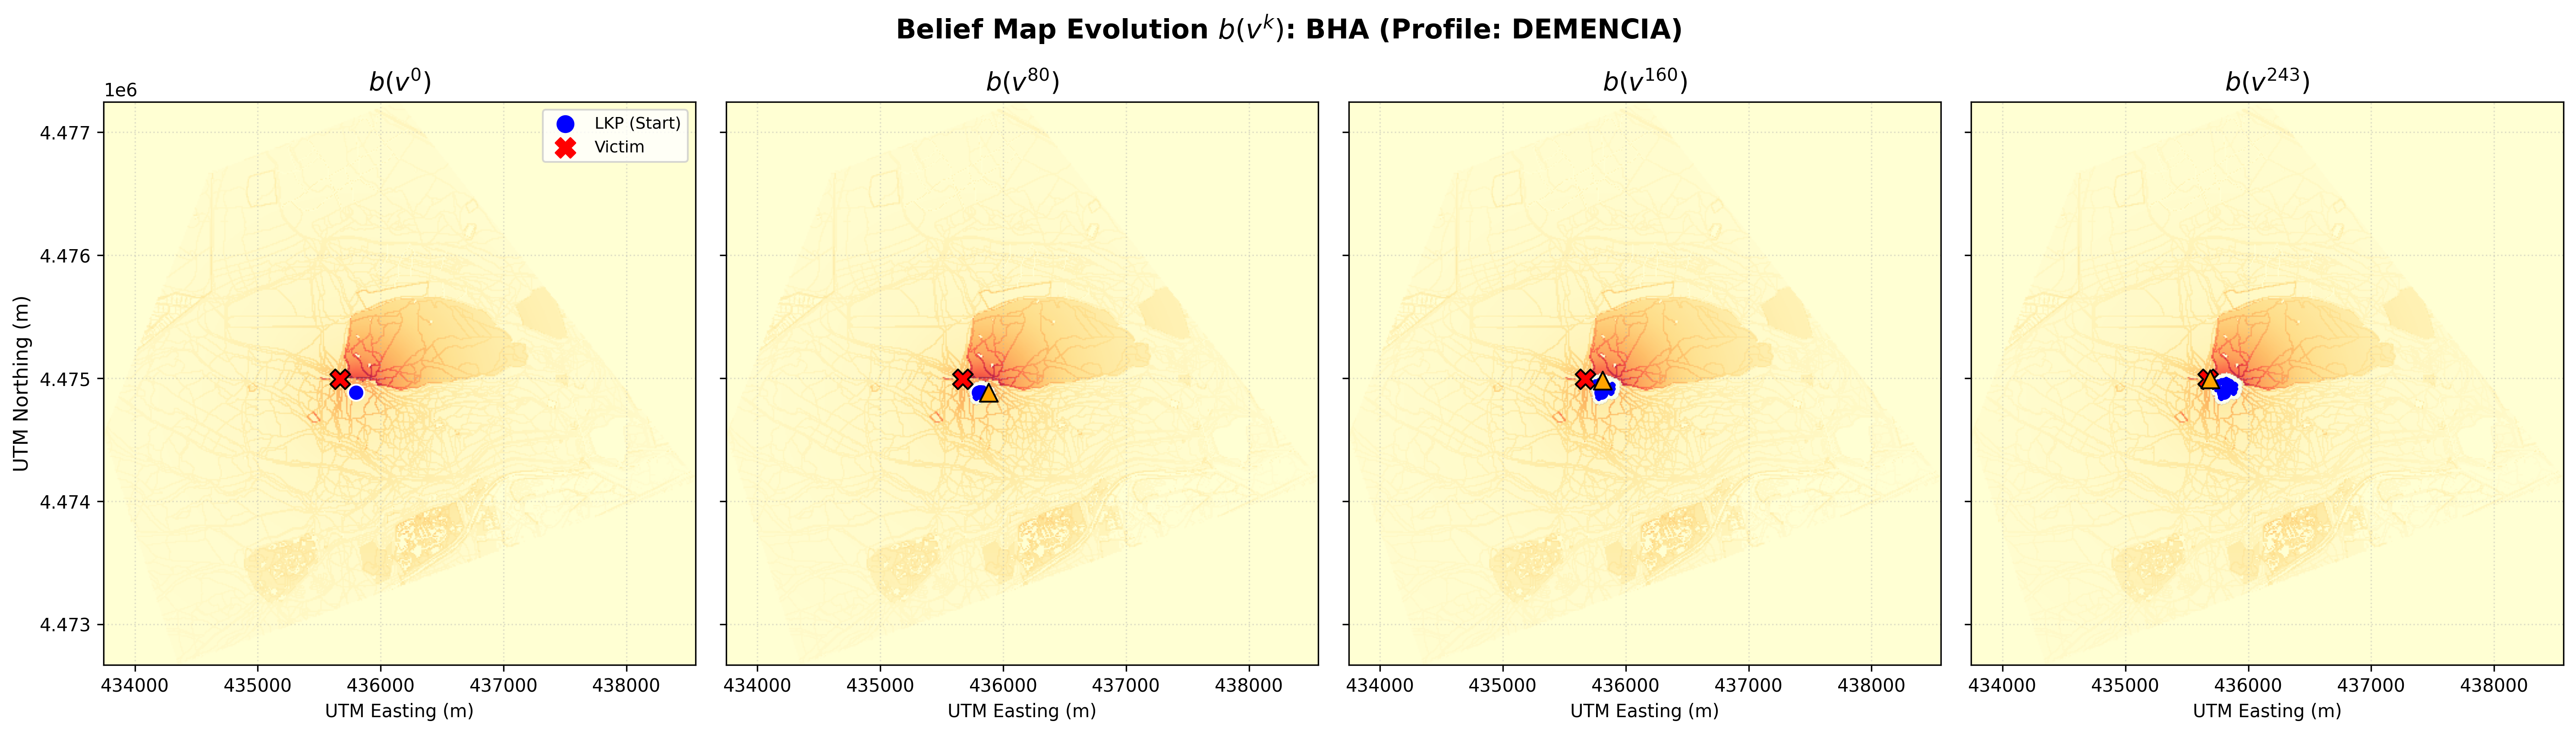
\includegraphics[width=0.95\textwidth]{imagenes/evolucion_temporal_demencia_bha.png}}
\end{figure}

El BHA exhibe una convergencia inicial significativamente más agresiva que el ABC. Al asignar al mejor candidato el papel de centro gravitatorio (\textit{black hole}), todas las soluciones estrella son atraídas rápidamente hacia el núcleo de mayor concentración probabilística. Esta aceleración permite al dron localizar e interceptar a la víctima de forma más temprana, alcanzando una aproximación de tan solo $20.2\text{ metros}$ en el paso $t=243$. Una vez que el dron absorbe la probabilidad central y el atractivo del agujero negro decae, las estrellas que cruzan el horizonte de sucesos son reemitidas estocásticamente a lo largo del dominio, generando una transición natural hacia un régimen exploratorio expansivo visible a $t=500$.

\subsection{Dinámica Espaciotemporal en el Perfil Autista: Evasión Activa de Obstáculos y Búsqueda en Corredores}

El perfil de personas en el espectro autista presenta una morfología espacial discontinua: aunque la literatura forense constata una atracción notable hacia elementos acuáticos y estructuras antrópicas, el módulo de restricciones físicas duras del framework anula por completo ($P=0.0$) el interior de láminas de agua (como el Lago de la Casa de Campo) y las geometrías de edificios cerrados para evitar colisiones o trayectorias inviables. En consecuencia, la masa de probabilidad se dispersa en racimos (\textit{clusters}) irregulares a lo largo de linderos, claros y márgenes transitables.

La Figura~\ref{fig:evolucion_autista_abc} ilustra el rastreo ejecutado por la Colonia de Abejas (ABC) para la Semilla~44.

\begin{figure}[H]
	\ffigbox[\FBwidth]
	{\caption{EVOLUCIÓN TEMPORAL DEL MAPA DE CREENCIAS RESIDUAL $b(v^k)$ EN EL PERFIL AUTISTA BAJO COLONIA DE ABEJAS (ABC, SEMILLA 44)}}
	{\label{fig:evolucion_autista_abc}
	
\includegraphics[width=0.95\textwidth]{imagenes/evolucion_temporal_autista_abc.png}}
\end{figure}

En la secuencia temporal se observa con claridad cómo las zonas vedadas permanecen como regiones oscuras de nula probabilidad durante toda la misión. El dron no desperdicia batería sobrevolando las aguas del lago; en su lugar, el gradiente bayesiano guía al enjambre hacia los parches boscosos adyacentes. A $t=100$, el UAV ya ha seleccionado el corredor con mayor acumulación de probabilidad periférica. La navegación adaptativa sortea las barreras físicas y consigue cerrar la aproximación a la víctima en el paso $t=315$, registrando una distancia crítica de apenas $20.5\text{ metros}$. En los instantes subsiguientes ($t=500$), el mapa de creencias evidencia una depresión casi total en el clúster objetivo, demostrando la alta selectividad espacial del método sin incurrir en maniobras de alto riesgo en zonas restringidas.

\subsection{Dinámica Espaciotemporal en el Perfil Senderista: Rastreo de Topologías Lineales y Análisis Crítico de la Búsqueda Voraz}

El perfil de Senderista constituye el escenario más polarizado del benchmark debido a su topología predominantemente unidimensional. Las personas extraviadas en esta categoría tienden a seguir la red de caminos, pistas forestales y sendas señalizadas de la Casa de Campo. 

La Figura~\ref{fig:evolucion_senderista_abc} expone el desempeño de la Colonia de Abejas (ABC) en este entorno para la Semilla~39.

\begin{figure}[H]
	\ffigbox[\FBwidth]
	{\caption{EVOLUCIÓN TEMPORAL DEL MAPA DE CREENCIAS RESIDUAL $b(v^k)$ EN EL PERFIL SENDERISTA BAJO COLONIA DE ABEJAS (ABC, SEMILLA 39)}}
	{\label{fig:evolucion_senderista_abc}
	
\includegraphics[width=0.95\textwidth]{imagenes/evolucion_temporal_senderista_abc.png}}
\end{figure}

Al encontrarse la probabilidad canalizada en filamentos estrechos, el ABC debe coordinar a sus agentes para no perder la traza del sendero. En la Semilla~39, la persona extraviada se encuentra en una bifurcación de caminos. Entre $t=100$ y $t=300$, el enjambre despliega patrullas a lo largo del eje troncal, explorando las ramas secundarias a medida que el filtro bayesiano extingue el tramo principal. La intercepción exitosa se produce en el paso $t=445$ a una distancia de $22.4\text{ metros}$, dejando a $t=500$ un canal continuo de probabilidad consumida que coincide con el trazado topográfico de OpenStreetMap.

Finalmente, la Figura~\ref{fig:evolucion_senderista_voraz} muestra la evolución bajo el planificador Voraz Heurístico para la Semilla~14, permitiendo contrastar la naturaleza de ambas aproximaciones.

\begin{figure}[H]
	\ffigbox[\FBwidth]
	{\caption{EVOLUCIÓN TEMPORAL DEL MAPA DE CREENCIAS RESIDUAL $b(v^k)$ EN EL PERFIL SENDERISTA BAJO VORAZ HEURÍSTICO (SEMILLA 14)}}
	{\label{fig:evolucion_senderista_voraz}
	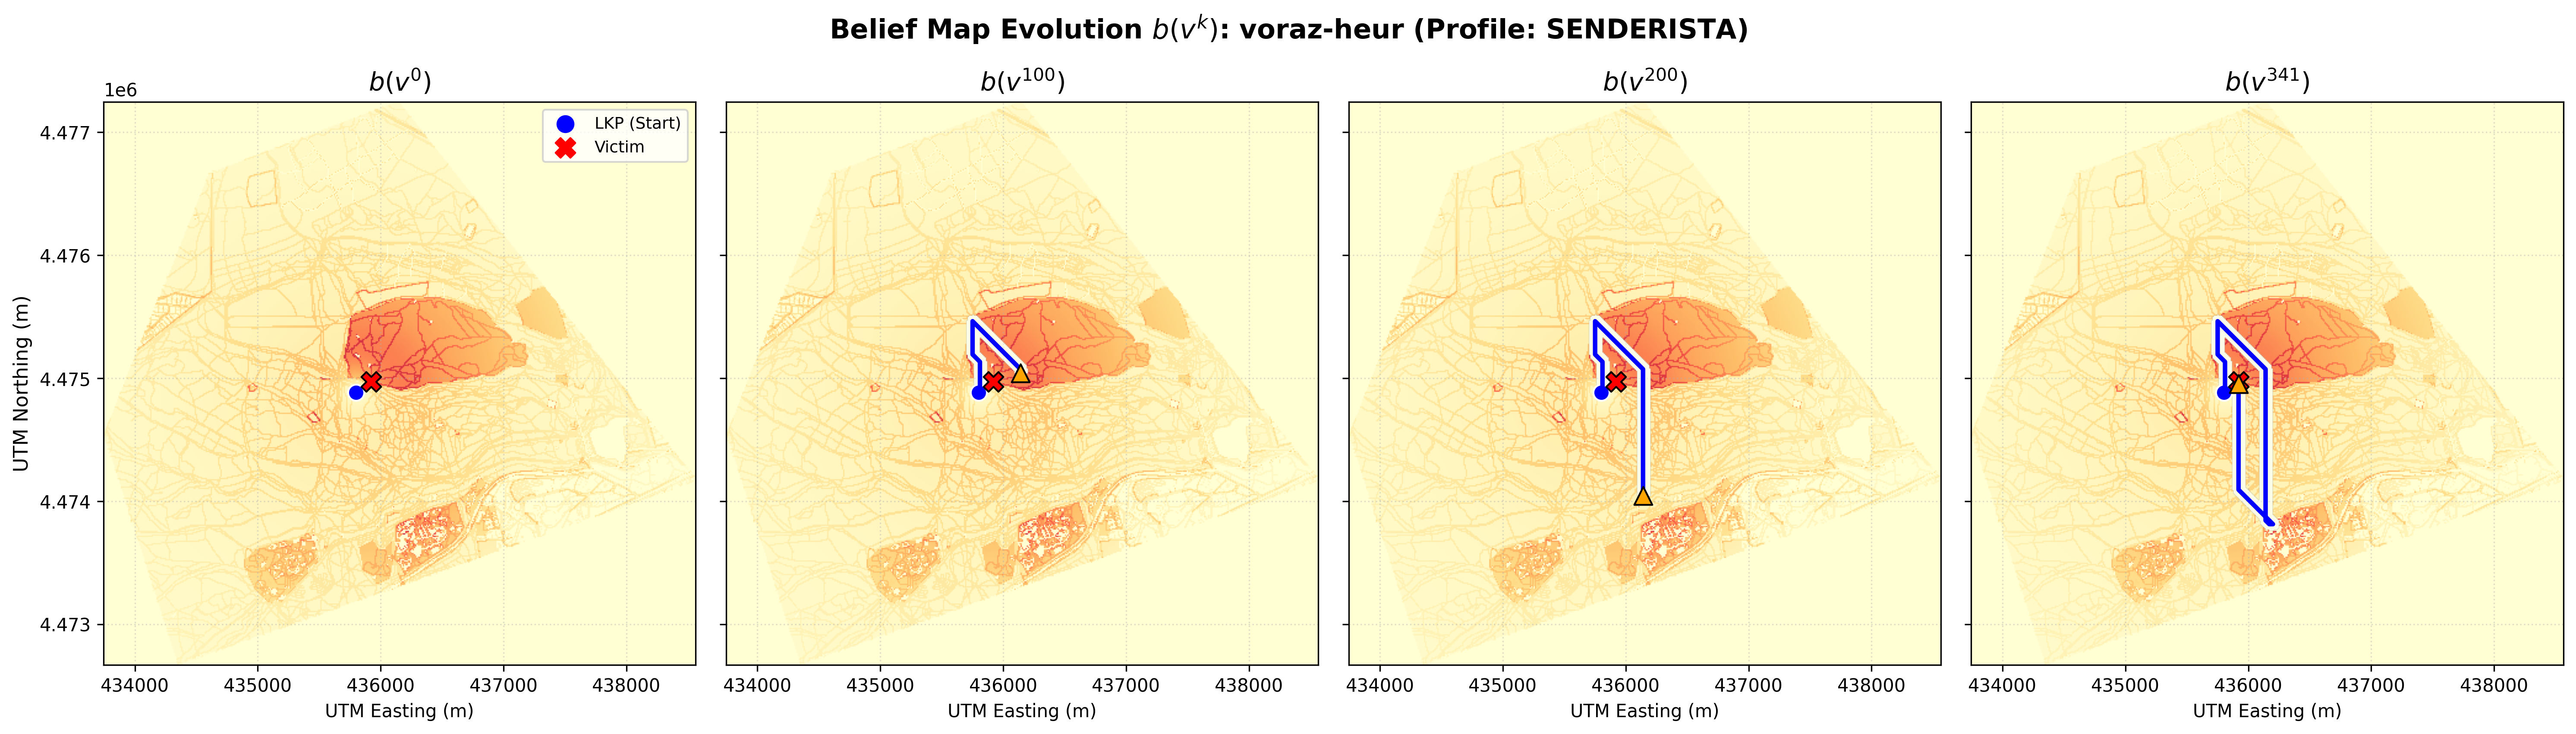
\includegraphics[width=0.95\textwidth]{imagenes/evolucion_temporal_senderista_voraz.png}}
\end{figure}

En redes lineales continuas, el algoritmo Voraz opera de forma análoga a un seguidor de líneas por gradiente ascendente: en cada paso escoge el avance que maximiza la absorción local instantánea de probabilidad. Cuando la víctima se encuentra situada a lo largo del sendero inicial (como en la Semilla~14), Voraz se desplaza con una celeridad implacable, alcanzando a la víctima en el paso $t=341$ a $20.3\text{ metros}$ de distancia. Sin embargo, la inspección minuciosa del mapa residual a $t=500$ revela la grave deficiencia estructural del método voraz: la aeronave consume un surco extremadamente angosto y, al llegar al término del camino o toparse con un claro desprovisto de probabilidad, se bloquea por completo o realiza giros erráticos, incapaz de cruzar zonas vacías para saltar a senderos paralelos. Este fenómeno explica por qué el Voraz Heurístico lidera la tasa de acierto en el perfil de Senderista ($13.01\%$), donde los senderos forman autovías de probabilidad continua, pero fracasa rotundamente en terrenos complejos y fragmentados como Demencia ($5.41\%$) o Autista ($4.89\%$), donde la visión global y la capacidad de escape de los algoritmos bioinspirados (ABC y BHA) resultan indispensables.

\section{Comparativa Global: Bioinspirados vs. Baselines Clásicos}

Para ilustrar la distribución estadística de las métricas en las 900 simulaciones, las Figuras~\ref{fig:box_acierto} y \ref{fig:box_distancia} muestran los diagramas de caja (\textit{boxplots}) comparativos de la tasa de acierto y la distancia de vuelo.

\begin{figure}[H]
	\ffigbox[\FBwidth]
	{\caption{COMPARATIVA DE LA TASA DE ÉXITO (\% ACIERTO) POR PERFIL DE BÚSQUEDA}}
	{\label{fig:box_acierto}
	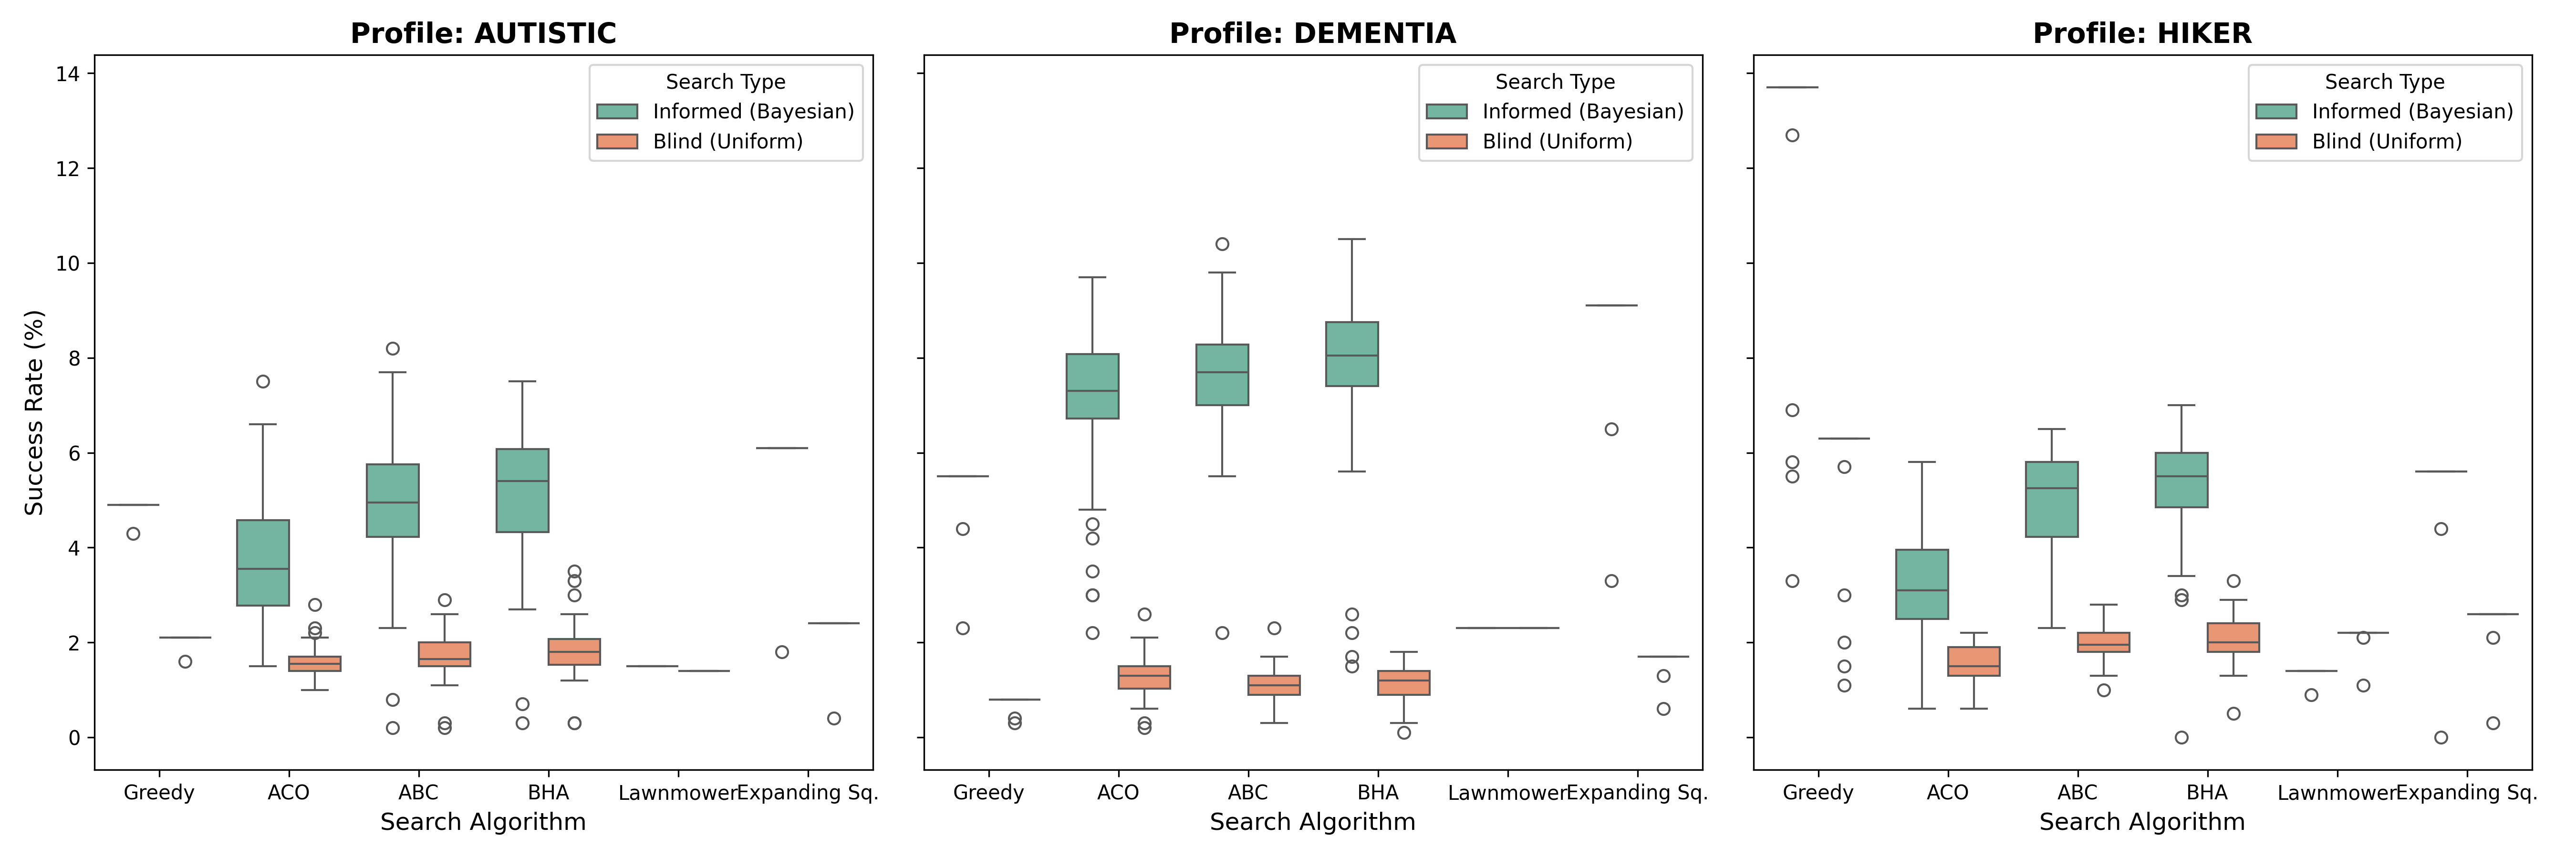
\includegraphics[width=0.90\textwidth]{imagenes/comparativa_acierto_perfiles.png}}
\end{figure}

\begin{figure}[H]
	\ffigbox[\FBwidth]
	{\caption{COMPARATIVA DE LA DISTANCIA TOTAL DE VUELO (KM) POR ALGORITMO}}
	{\label{fig:box_distancia}
	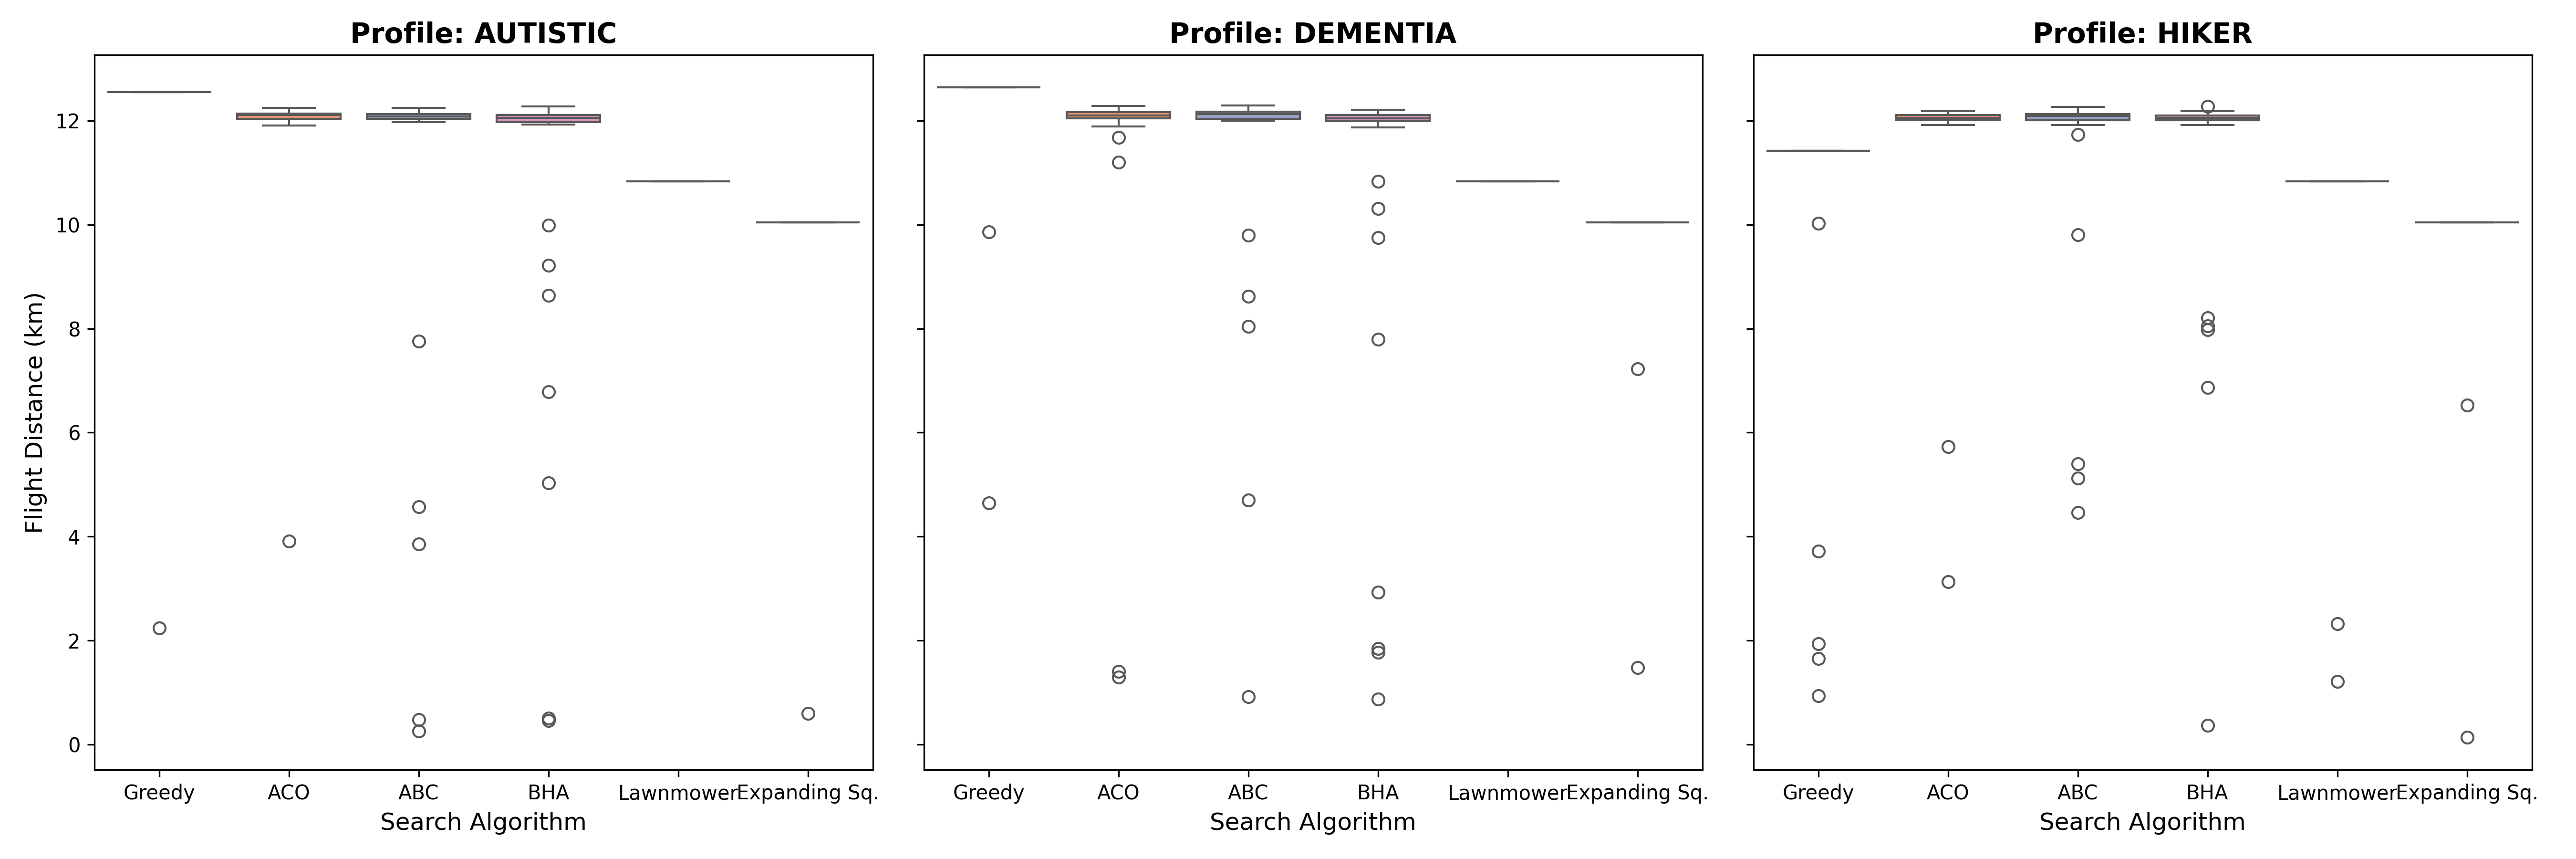
\includegraphics[width=0.90\textwidth]{imagenes/comparativa_distancia_perfiles.png}}
\end{figure}

\subsection{Discusión de la Eficiencia Operativa y Energética}

El análisis cruzado de las cinco métricas consolidadas en el benchmark revela cuatro conclusiones fundamentales:

\begin{enumerate}
    \item \textbf{Superioridad Drástica de la Búsqueda Informada:} En todos los perfiles evaluados, la disponibilidad del mapa de calor bayesiano multiplica la probabilidad de rescate entre 3x y 6x respecto a la búsqueda ciega con el mismo presupuesto de batería.
    \item \textbf{Inutilidad Operativa del Barrido Lawnmower:} Aunque el patrón de cortacésped maximiza la superficie geográfica barrida ($A_{\text{cov}} = 0.848\text{ km}^2$), obtiene la peor tasa de éxito ($1.39\% - 2.30\%$) debido a que dispersa la escasa energía del UAV sobre grandes extensiones de terreno con probabilidad nula.
    \item \textbf{Equilibrio Óptimo de ABC y BHA:} Las metaheurísticas bioinspiradas logran la mayor concentración de probabilidad reducida ($P_{\text{red}}$) con trayectorias suaves de $11.0 - 11.6\text{ km}$, maximizando la probabilidad de supervivencia de la víctima durante los primeros 25 minutos críticos de la operación SAR.
    \item \textbf{Coste Computacional vs. Eficacia Táctica:} Desde la perspectiva de la computación, los patrones rígidos clásicos (\textit{Lawnmower} y \textit{Expanding Spiral}) poseen un tiempo de cálculo prácticamente nulo ($t_{\text{calc}} \approx 0\text{ s}$) al basarse en ecuaciones geométricas directas. En contrapartida, las metaheurísticas bioinspiradas (ACO, ABC y BHA), calibradas óptimamente mediante Optuna, requieren una fase previa de cálculo iterativo que oscila entre pocos segundos y escasos minutos en una estación de trabajo convencional. Operativamente, en una misión de salvamento donde la vida humana depende de la celeridad del rescate, aguardar 30 o 60 segundos en el puesto de mando avanzado antes del despegue para computar una ruta optimizada que multiplica por hasta seis veces la probabilidad de éxito representa un coste computacional plenamente asumible y altamente ventajoso.
\end{enumerate}

\subsection{Contextualización de la Escala Física y la Tasa de Éxito Absoluta}

Es fundamental interpretar con rigor de ingeniería los valores porcentuales absolutos obtenidos en las tasas de acierto ($5.0\% - 13.0\%$). En una inspección superficial, un lector no habituado al rescate en grandes masas forestales podría cuestionar por qué las tasas de acierto no alcanzan valores del $80\%$ o $90\%$. La explicación es que \textbf{estos órdenes de magnitud son plenamente esperables, naturales y coherentes con la física real del problema}, respondiendo a la conjunción de tres factores determinantes:

\begin{itemize}
    \item \textbf{La Inmensidad del Escenario (1.722 Hectáreas):} El parque de la Casa de Campo abarca más de $12.75\text{ km}^2$ de superficie operativa continua ($1.722\text{ hectáreas}$ de masa forestal y relieve agreste, 5 veces Central Park). Frente a esta enorme extensión geográfica, el dron vuela con una cámara óptica cenital que proyecta una huella circular de apenas $50\text{ metros}$ de radio ($0.0078\text{ km}^2$ de área instantánea).
    \item \textbf{La Restricción de un Único Dron y una Sola Batería de 25 Minutos:} Las 900 misiones evalúan el desempeño estricto de \textbf{un único UAV} dotado de \textbf{una sola batería de 25 minutos} ($250$ pasos de avance físico). En ese breve lapso temporal, un solo dron solo tiene capacidad física para sobrevolar entre un $1.5\%$ y un $3.5\%$ de la superficie total del parque. Pretender cubrir el parque entero con una única aeronave y una sola batería es físicamente imposible.
    \item \textbf{Dispersión Espacial Realista de las Víctimas:} Las 50 ubicaciones estocásticas de Montecarlo por perfil sitúan a la víctima en un radio de dispersión empírico de hasta varios kilómetros desde el punto de despegue (LKP).
\end{itemize}

Bajo estas restricciones físicas extremas, que \textbf{un único dron con una sola batería} localice directamente a la víctima en hasta el $13\%$ de los vuelos individuales en su primera salida confirma una capacidad sobresaliente de focalización guiada por el mapa bayesiano (frente al ínfimo $1.39\%$ del barrido ciego). En un dispositivo de emergencia real, la operación nunca concluye tras el primer vuelo: se despliegan cuadrillas de 3 a 6 drones simultáneos o se programan rotaciones consecutivas de cambio de batería, con lo cual la probabilidad acumulada de éxito escala de forma rápida hacia el $70\% - 90\%$ durante las primeras dos horas de rastreo.

\chapter{Conclusiones y Trabajo Futuro}
\label{cap:conclusiones}

En este capítulo final se sintetizan las principales aportaciones científicas y técnicas desarrolladas a lo largo de este Trabajo de Fin de Máster, se discuten las limitaciones asumidas durante el modelado y se plantean las líneas prioritarias de investigación futura.

\section{Conclusiones Principales}

El presente trabajo ha desarrollado e integrado con éxito un framework completo y unificado para la optimización de operaciones de búsqueda y rescate (SAR) mediante vehículos aéreos no tripulados (UAVs) sobre escenarios topográficos reales en entornos de incertidumbre:

\begin{enumerate}
    \item \textbf{Integración Topológica y Probabilística Realista:} Se ha superado la dependencia tradicional de mapas sintéticos simplificados mediante la conexión directa con OpenStreetMap (OSM) y la parametrización de perfiles canónicos del manual de comportamiento de personas desaparecidas (\textit{Lost Person Behavior} - LPB de Robert Koester).
    \item \textbf{Filtrado de Restricciones Físicas de Transitabilidad:} La incorporación de máscaras espaciales jerárquicas con árboles R-Tree ha permitido anular estrictamente la probabilidad ($P=0.0$) en zonas no transitables (lagos y edificaciones cerradas), eliminando falsos positivos en la asignación de recursos aéreos.
    \item \textbf{Arquitectura Modular y Portabilidad (`sarenv-mts`):} Se ha establecido una pasarela middleware que transforma las coordenadas globales UTM ($\text{EPSG:32630}$) en matrices discretas operables por el motor de búsqueda MTS, junto con un evaluador estandarizado de métricas SAR (\texttt{PathEvaluatorTFM}).
    \item \textbf{Calibración Bayesiana y Eficacia de Algoritmos Bioinspirados:} A través de un exhaustivo benchmark de 900 simulaciones de Montecarlo calibradas con Optuna, se ha demostrado cuantitativamente que los planificadores metaheurísticos bioinspirados (en particular la Colonia de Abejas Artificiales - ABC y el Algoritmo de Agujeros Negros - BHA) superan sistemáticamente a los patrones de barrido geométrico ciego (Lawnmower) y a la búsqueda voraz miope, logrando una reducción significativa en los tiempos de respuesta y una mayor concentración en áreas de alta verosimilitud.
\end{enumerate}

\section{Limitaciones del Trabajo}

A pesar de la consistencia metodológica del framework desarrollado, es necesario explicitar las siguientes limitaciones asumidas en la investigación:

\begin{enumerate}
    \item \textbf{Ausencia de Penalización Física en el Vector de Control Cinemático:} 
    Las restricciones físicas de no transitabilidad (masas de agua y edificaciones) se han aplicado como una \textit{restricción dura de probabilidad inicial} ($b(v^0) = 0.0$), garantizando que los planificadores no concentren esfuerzos de búsqueda en dichas zonas. Sin embargo, no se ha incorporado un término de repulsión cinemática en las acciones de vuelo del UAV, permitiendo que el dron pueda sobrevolar en línea recta masas de agua durante su desplazamiento hacia otras regiones de alta probabilidad.

    \item \textbf{Asunción de Víctimas Estáticas en la Batería Experimental:} 
    Las 900 simulaciones del benchmark consideran que la persona desaparecida permanece en una ubicación fija e inalterable desde el inicio de la misión hasta su hallazgo o el agotamiento de la autonomía de vuelo.
\end{enumerate}

\section{Líneas de Trabajo Futuro}

Como extensión directa de los resultados y la arquitectura desarrollada, se plantean las siguientes líneas de trabajo futuro:

\begin{itemize}
    \item \textbf{Integración Operativa Aire-Tierra y Validación con Simulacros Reales de Bomberos:} 
    El escenario seleccionado en este trabajo (Casa de Campo de Madrid) responde a un ejercicio operativo real de búsqueda y salvamento coordinado por cuerpos de bomberos y protección civil, del cual se dispone de la sectorización territorial, la ubicación del Puesto de Mando Avanzado (PMA) y los registros de posicionamiento GPS (\textit{tracks} GPX) de 12 equipos de batida terrestre. Como continuación directa, se plantea articular una arquitectura colaborativa multinivel que combine dos escalas operativas:
    \begin{itemize}
        \item \textit{Escala Macro (Exploración Aérea Temprana):} El UAV opera a $10\text{ m/s}$ ($36\text{ km/h}$) a $50\text{ m}$ de altitud como vector táctico de detección rápida sobre el macro-escenario completo. Su cometido prioritario es absorber la mayor masa de creencia bayesiana en los primeros 15--20 minutos, transmitiendo las coordenadas del contacto o las zonas de máxima certidumbre al PMA para focalizar el despliegue de los recursos a pie.
        \item \textit{Escala Micro (Validación y Batida Sectorizada):} Restringir los algoritmos bioinspirados de \texttt{sarenv-mts} al polígono específico de uno de los subsectores asignados a los bomberos para contrastar cuantitativamente la trayectoria y el tiempo de cobertura del dron frente a la traza GPX registrada a pie por el equipo terrestre ($3\text{--}4\text{ km/h}$). Asimismo, cruzar el mapa de creencia residual $b(v^k)$ con las áreas batidas por los rescatadores a pie permitirá optimizar la reasignación dinámica de cuadrantes y eliminar búsquedas redundantes.
    \end{itemize}
    
    \item \textbf{Modelado de Víctimas Dinámicas mediante Cadenas de Markov y Random Walk:} 
    Incorporar matrices de transición dinámicas $P(x, y, t)$ orientadas por la pendiente del terreno, senderos y perfiles psicológicos de dispersión extraídos del Manual de Búsqueda y Salvamento Terrestre \cite{romero2018manual}.
    
    \item \textbf{Control de Vuelo Guiado por Campos Potenciales de Repulsión:} 
    Implementar restricciones cinemáticas de no sobrevuelo en la capa de bajo nivel del UAV para impedir físicamente que el dron cruce masas de agua o zonas de exclusión aérea.
\end{itemize}



%----------
%	BIBLIOGRAFÍA
%----------	

\nocite{*} % Si quieres que aparezcan en la bibliografía todos los documentos que la componen (también los que no estén citados en el texto) descomenta está línea

\clearpage
\addcontentsline{toc}{chapter}{Bibliografía}
\setquotestyle[english]{british} % Cambiamos el tipo de cita porque en el estilo IEEE se usan las comillas inglesas.
\printbibliography



%----------
%	ANEXOS
%----------	

% Si tu trabajo incluye anexos, puedes descomentar las siguientes líneas
%\chapter* {Anexo x}
%\pagenumbering{gobble} % Las páginas de los anexos no se numeran



\end{document}